% -*-latex-*-

\chapter{Helicity Decoder}
\label{A1}

In \Cref{C5S1SS2}, we have discussed the helicity scheme of E08-027. During the experiment, the helicity scheme was determined by the Hall C QWEAK experiment with a high reversal rate at 960.02 Hz. The typical DAQ rate of E08-027 was $5\sim6$ kHz. The helicity decoder for QWEAK helicity scheme (THaQWEAKHelicity in the Hall A analyzer package) requires the DAQ rate to be lower than 100 Hz \cite{Hansen2015}, thus this decoder could not be used in E08-027. A new helicity decoder was designed for E08-027. In this section, we will discuss the algorithm used by this new decoder and the test results. This section is also available as a technical note, Ref. \cite{Gu2014}.

\section{Data Acquisition Setup}
\label{A1S1}

To calculate the asymmetry, each recorded event needs to be sorted by the helicity of the electron beam. The number of accepted events in each helicity state is normalized by the total charge from BCM and the DAQ live time with the same helicity. Thus, the BCM signal, the triggers (T1$\sim$T8) and L1A signal of Hall A DAQ need to be sorted by the beam helicity. In E08-027, these signals and the detected physical events are addressed as two different issues.

The helicity signals described in \Cref{C5S1SS2} are copied to three different electronics during E08-027. The helicity of the physical event is recorded by the trigger interface (TI). The TI has 12 state registers (TIR). Four of these registers are used to record all of the four helicity signals, Pattern Sync, Pair Sync, Delayed Helicity and $\tsettles$, respectively (See \Cref{C5S1SS2F1}). The electronics setup is based on Ref. \cite{Michaels2010} and the recorded helicity is referred as TIR helicity in the rest of this section. Besides, decoding the TIR helicity requires timing information. The standard 103.7 kHz fast clock signal of Hall A was used to set a time-stamp for each physical event.

The BCM signals, triggers and L1A signals are all pulse signals. Helicity-gated SIS3801 scalers are used in the experiment to count these signals. \Cref{A1S1F1} shows the workflow of a SIS3801 scaler. The scaler contains 32 data registers to count, 8 control registers and a FIFO (First-In-First-Out) data buffer. The data signals are sent to the data registers and the $\tsettles$ signal is sent to one of the control registers to make a veto gate. The data registers only count during the $\tstable$ part of a helicity window. Once the counting of one helicity window is finished, the FIFO reads the counting results and save them temporarily. Two additional control registers are used to record the Delayed Helicity and Pattern Sync signals. The FIFO also reads these and records the helicity state of each helicity window.

\begin{figure}[tb!]
  \centering
  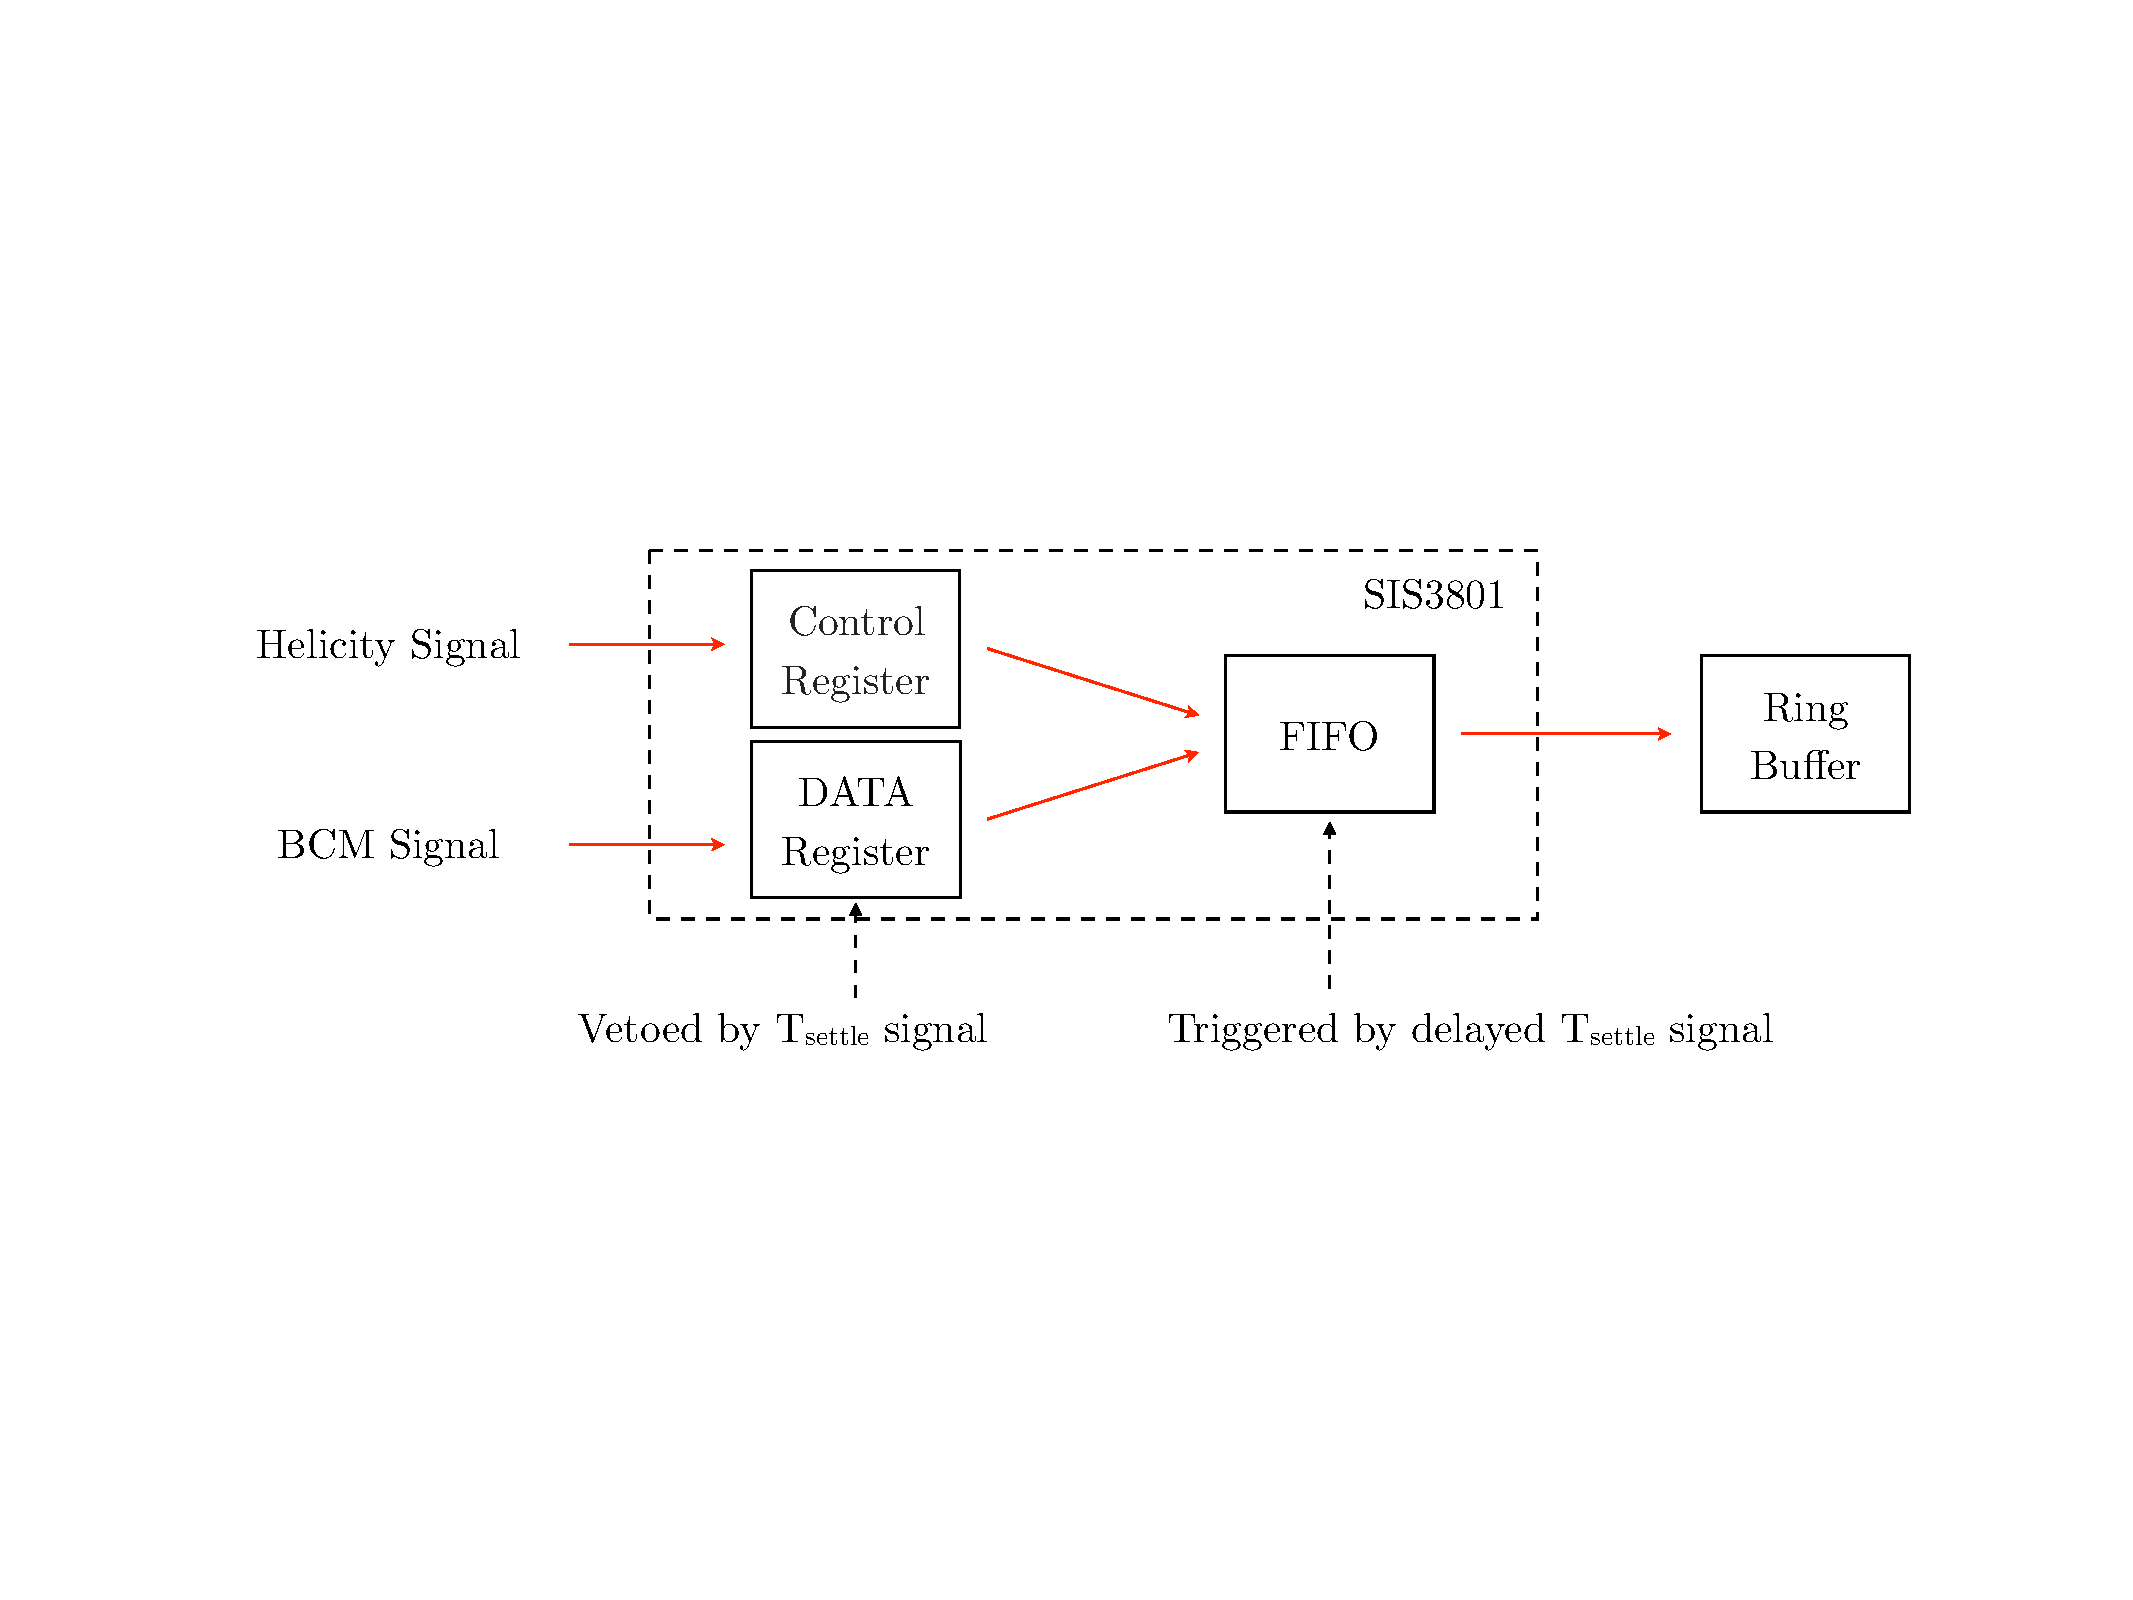
\includegraphics[width=0.9\textwidth]{figs/sis3801.pdf}
  \caption{Workflow of a SIS3801 scaler. \label{A1S1F1}}
\end{figure}

However, the FIFO is not capable to store a large amount of data. A ring buffer, which is able to store the counting results of 1000 helicity windows, is set in the memory of the VME crate to keep the counting results. The ring buffer is read by the DAQ system every 50 physical events to reduce DAQ dead time. After each readout, the ring buffer is cleared for new counting results. With SIS3801 scalers, the helicity-gated counting results are saved to the raw data file marked with their helicity. The helicity recorded by the ring buffer is referred as ring buffer helicity hereafter.

\section{Helicity Decoder}
\label{A1S2}

As mentioned in \Cref{C5S1SS2}, the helicity recorded by the DAQ of experimental halls is delayed by 8 helicity windows compare to the actual helicity of the beam. In the accelerator injector, the beam helicity is determined by a pseudo-random generator which is shown in \Cref{A1S2F1}. Since the algorithm of this pseudo-random generator is well defined, the actual helicity can be extracted via the same pseudo-random algorithm. The idea is to read 30 continuous helicity quartets to retrieve the random seed, and use this seed to predict the reported helicity, i.e. the delayed helicity as well as the actual helicity. The prediction can be compared to the reported helicity of the first window of each pattern in the helicity sequence to make sure it is correct.

\begin{figure}[b!]
  \centering
  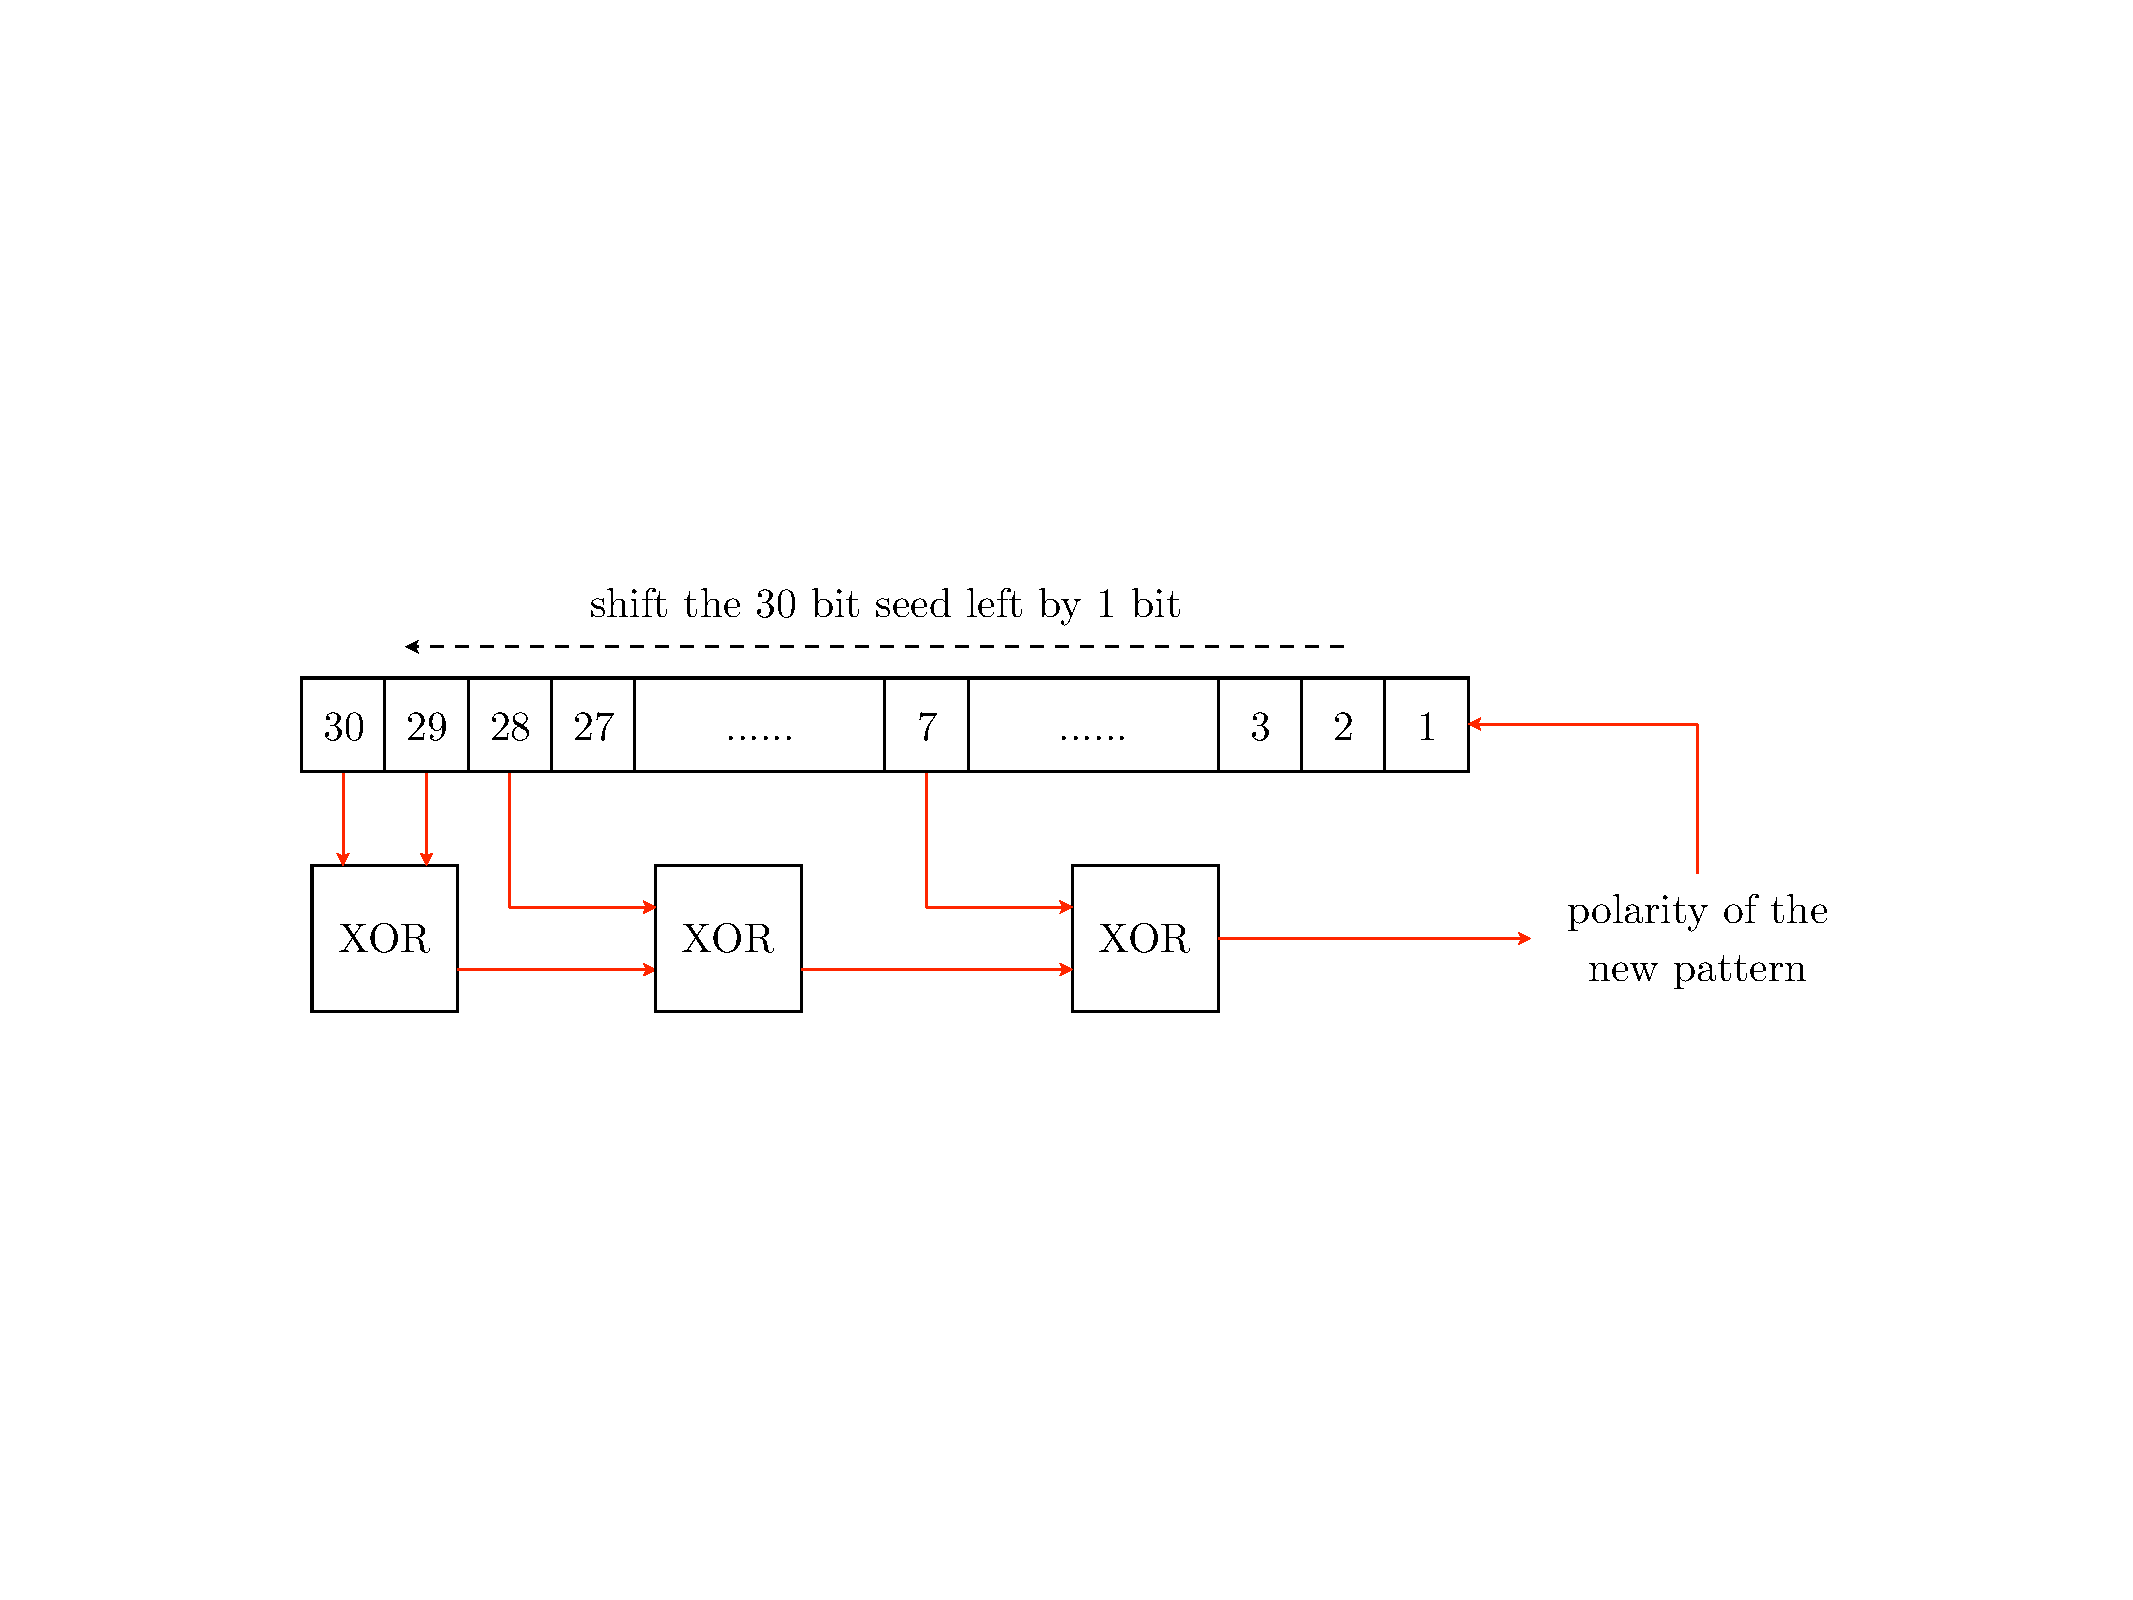
\includegraphics[width=0.8\textwidth]{figs/helicity-pseudo-random.pdf}
  \caption[The pseudo-random generator of the helicity signal.]{The 30-bit shift register in the Helicity Control Board. The polarity of a new quartet is calculated by applying an XOR (exclusive disjunction) operation to the bit 30, bit 29, bit 28 and bit 7 of a 30-bit register. Then the register is left-shifted by one bit and the new bit 1 is set by the XOR result. The repeat length of this generator is $2^{30} - 1 = 1,073,741,823$ bits. \label{A1S2F1}}
\end{figure}

\subsection{Predict Actual Ring Buffer Helicity}
\label{A1S2SS1}

The ring buffer saves a full sequence of the helicity as mentioned in \Cref{A1S1}. The sequence breaks only if no event was written during the time period of 1000 helicity windows that in our case is about a second. This is because the capacity of the ring buffer is 1000 helicity windows, and the newly coming data flush the old one out if the DAQ system does not read the ring buffer to clear it.

The method of decoding the ring buffer helicity is shown in \Cref{A1S2SS1F1}. If the random seed is not set, the program reads the ring buffer helicity in sequence and selects out the windows with Pattern Sync 1. The helicities of these windows are appended to the random seed. The seed is used to predict the reported helicity and the actual helicity of the next helicity pattern once all 30 bits are collected. For a Quartet pattern (``$+--\,+$'' or ``$-++\,-$''), only the helicity of the first window needs to be predicted by the seed, because the helicities of the second and the third windows of the quartet are always opposite to the first window and the helicity of the forth window is always equal to the first one. After prediction of all four windows in one quartet, the random seed is left-shifted by one bit and the new bit 1 is set with the reported helicity of the first window of the predicted pattern. The prediction is verified with the reported helicity sequence. If the prediction does not agree with the reported value for any reason, all windows in this quartet are marked as bad and the 30-bit random seed is reset immediately and generate again.

\begin{figure}[tb!]
  \centering
  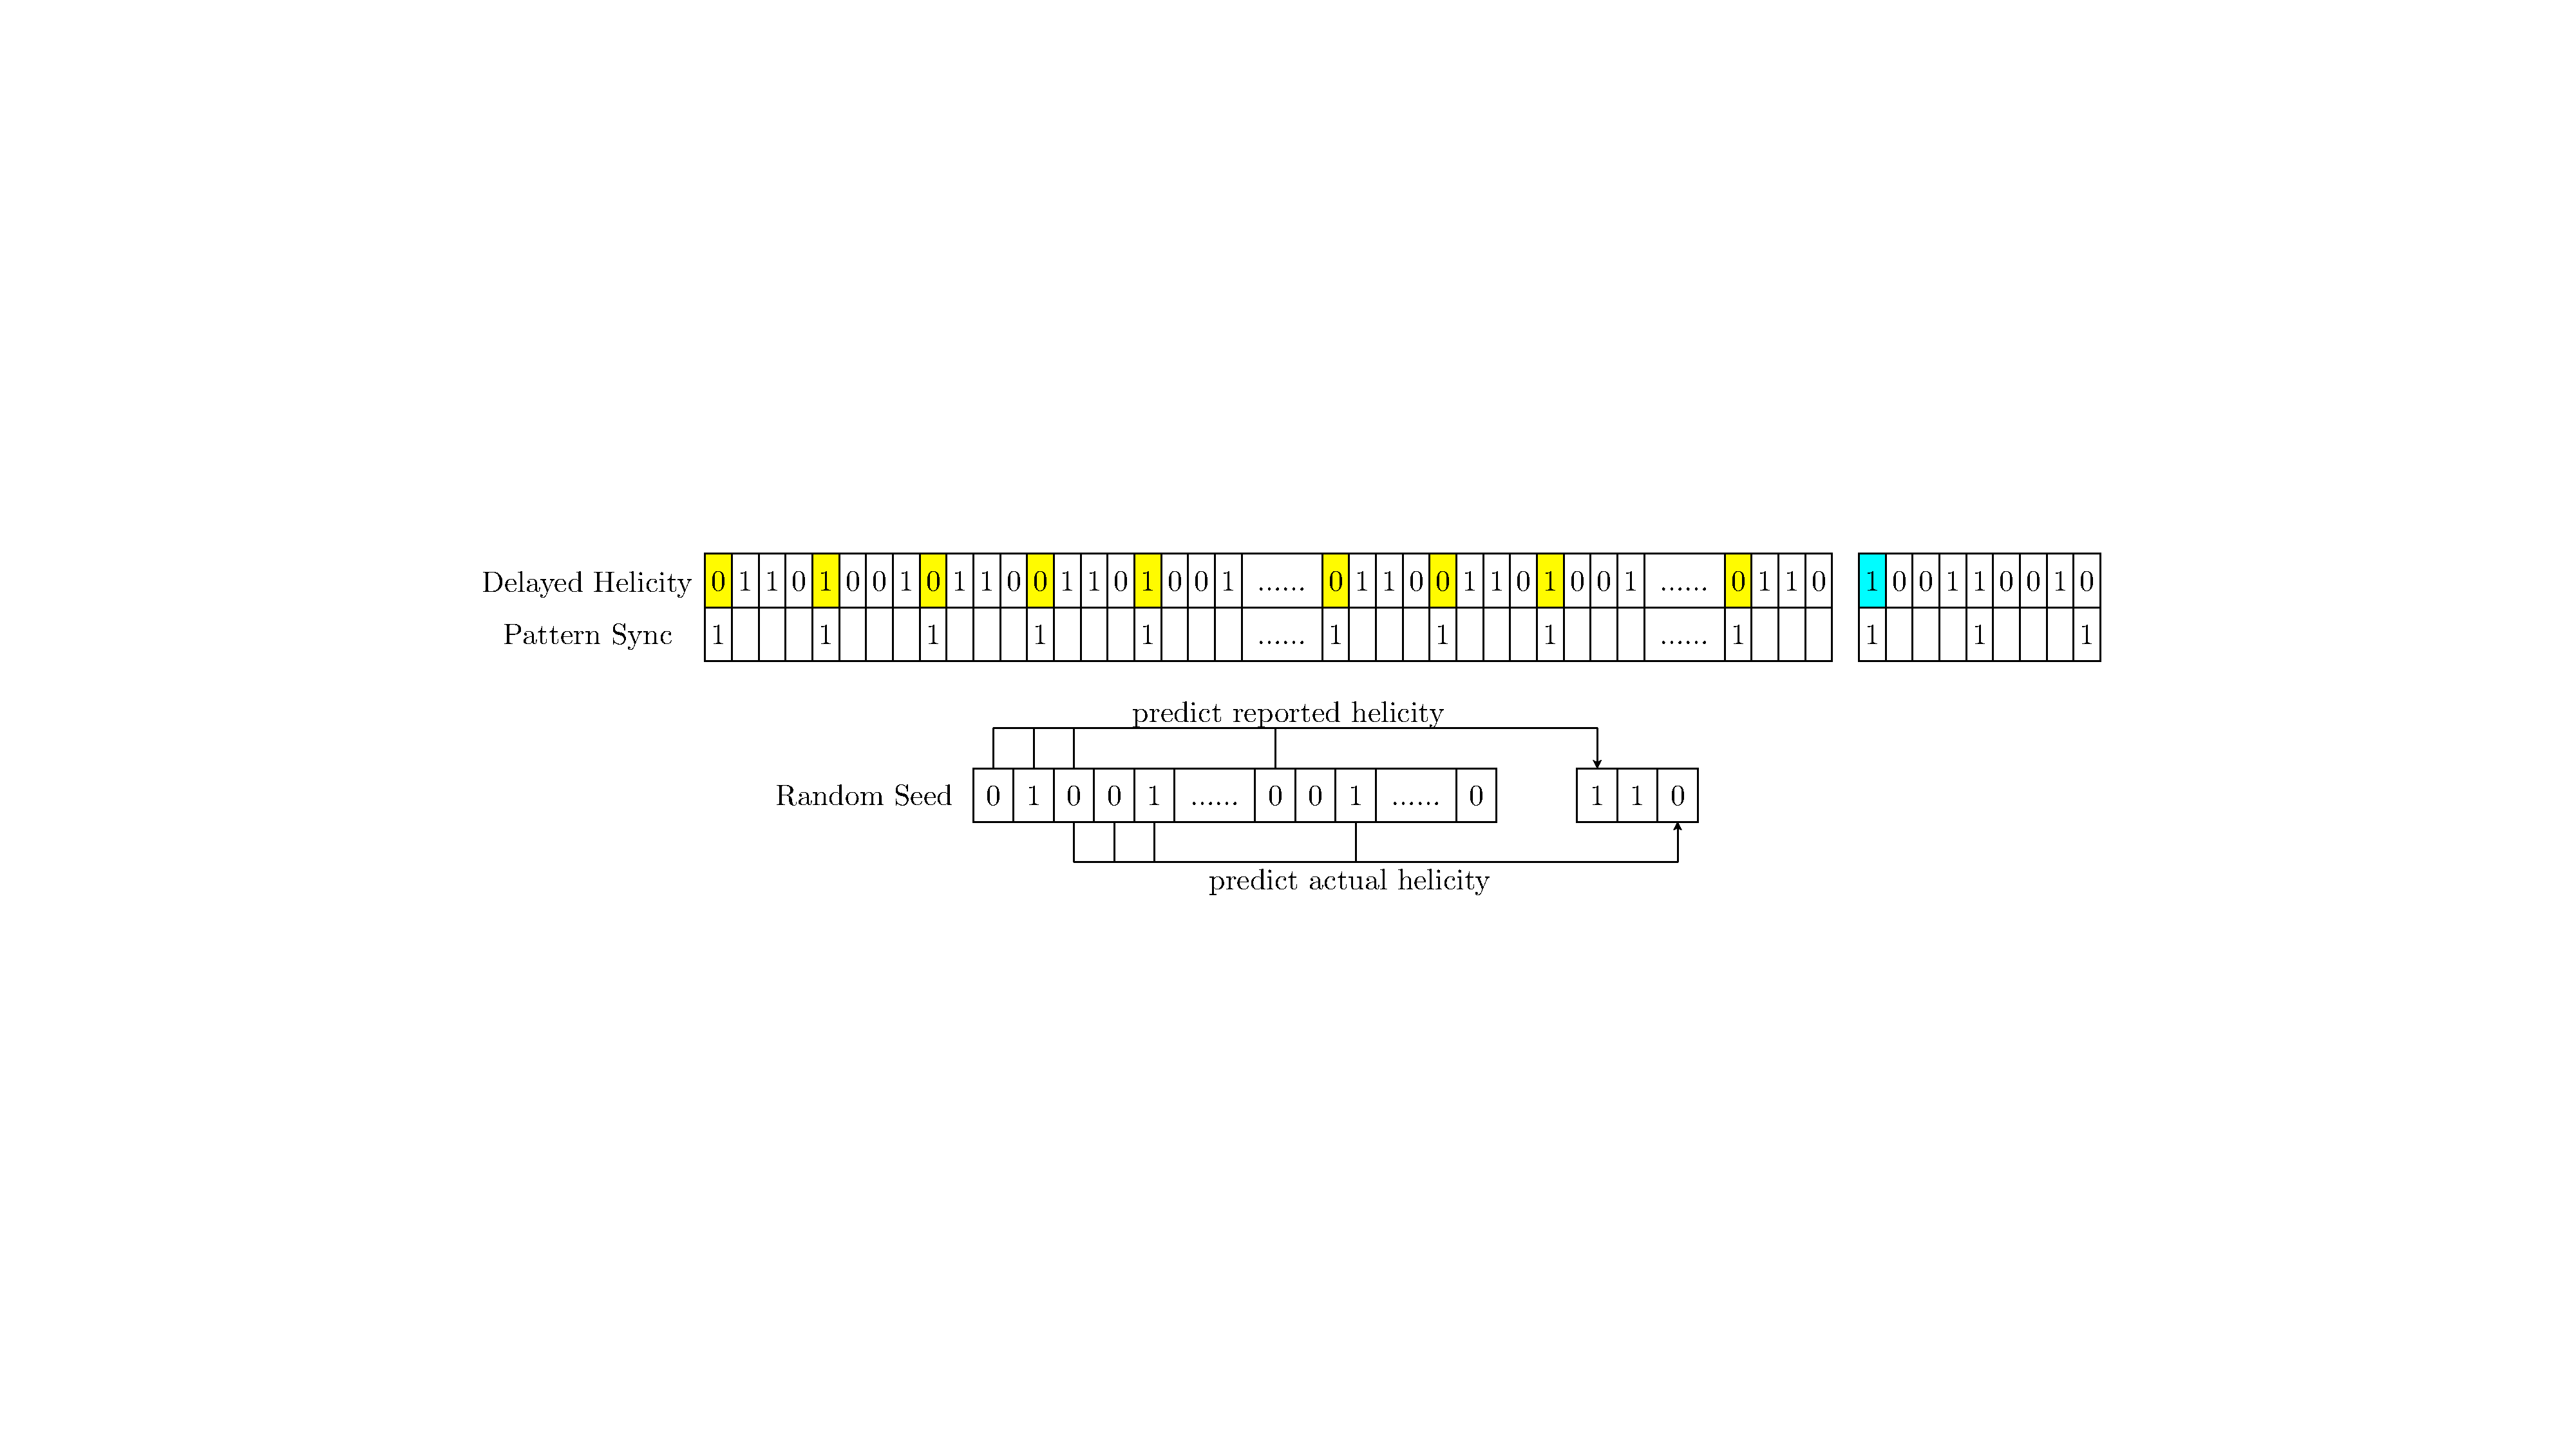
\includegraphics[width=\textwidth]{figs/ring-buffer-helicity.pdf}
  \caption[Predict actual ring buffer helicity.]{Predict actual ring buffer helicity. The windows marked as yellow are used to generate the random seed. The seed is used to predict the reported helicity and the actual helicity of the newly coming window (marked as cyan), using the 30-bit shift register algorithm shown in \Cref{A1S2F1}. The actual helicity is behind the reported one by 2 quartets or 8 helicity windows. In this example, the reported helicity of the cyan window is 1 but the actual helicity is 0. \label{A1S2SS1F1}}
\end{figure}

\subsection{Predict Actual TIR Helicity}
\label{A1S2SS2}

For TIR helicity, the decoding algorithm is still based on the prediction method. However, it is possible that several raw events are saved in one helicity window, or no physical event is saved during several helicity windows. \Cref{A1S2SS2F1} shows an example of TIR helicity. It does not show any obvious pattern, which makes the decoding more difficult. It is critical to find a method to locate each event in the helicity sequence before any prediction can be proceed. Since the helicity windows all have identical time length, it is possible to identify each raw event in the helicity sequence if they are labeled by some kind of time-stamp. The standard 103.9 kHz fast clock signal of Hall A was used to set the time-stamp during the experiment. The clock signal is counted by an ungated scaler (which means it is not helicity gated), and read by the DAQ system for each event. The helicity reversal frequency is 960.02 Hz in the experiment, so the time length of each window is about $\tw=103900\divisionsymbol960.02\approx108.2$ scaler counts. Some of the TIR event may be saved during the $\tsettle$ part of a helicity window. These events were excluded from the decoding process and marked as ``unstable'' by the decoder.

\begin{figure}[tb!]
  \centering
  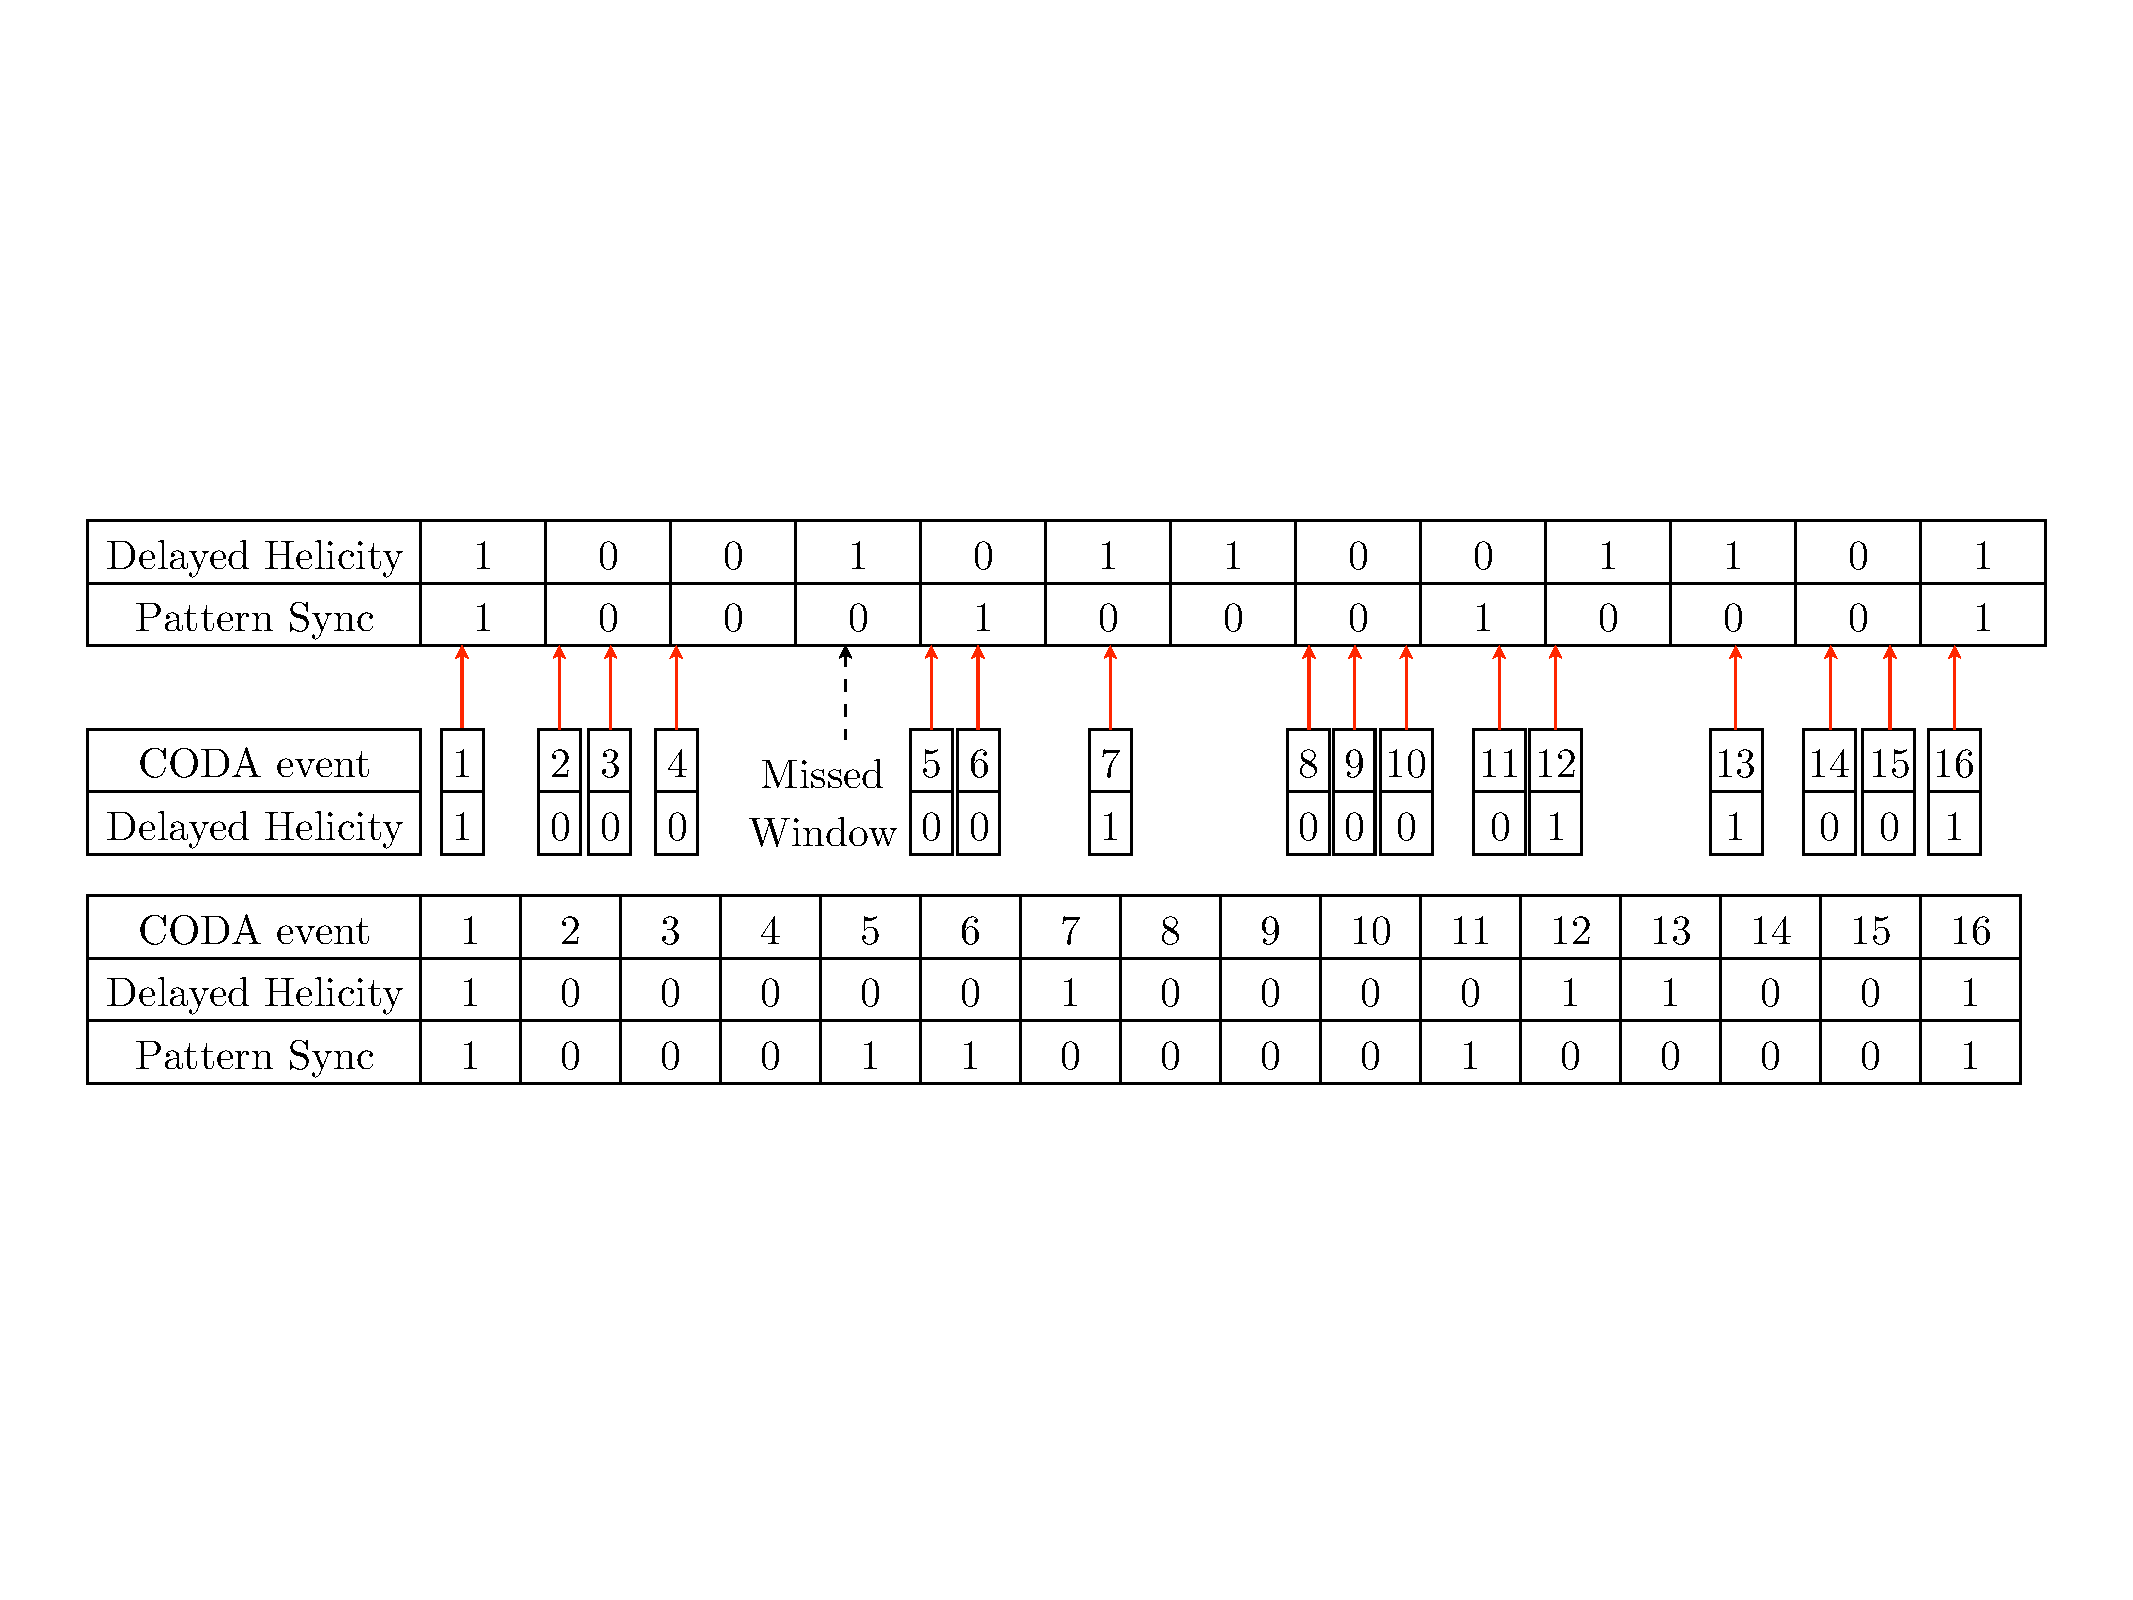
\includegraphics[width=\textwidth]{figs/tir-helicity.pdf}
  \caption[An example of the TIR helicity.]{An example of the TIR helicity. The sequence on the top is the normal helicity sequence. The physical event stream at the bottom shows how the TIR helicity breaks the normal helicity sequence. \label{A1S2SS2F1}}
\end{figure}

The first step to decode the TIR helicity is still to generate the random seed. For convenience, the helicity windows with Pattern Sync 1 are referred as Pattern Sync windows hereafter. Any events in these Pattern Sync windows are also referred as Pattern Sync events. The helicity of Pattern Sync events is used to generate the random seed, however, there are 3 different situations for the TIR helicity:
\begin{enumerate}[parsep=0pt]
\item \label{A1S2SS2A1} The event is the first event of a Pattern Sync window, and no Pattern Sync window is missed before this event. In this case, the helicity of this event should be appended to the random seed.
\item The event is the second (or third, ...) event of a Pattern Sync window. In this case it is ignored because the first event of this window has been appended to the random seed.
\item \label{A1S2SS2A2} The event is the first event of a Pattern Sync window, but one or more Pattern Sync windows are missed before this event. In this case, all existed 30 bits of the random seed are reset.
\end{enumerate}
In the decoder, a time interval $\dtpat$ is calculated to determine these 3 situations. Assuming the time-stamp of the current event is $T$ and the previous Pattern Sync event is $\tlastpat$, $\dtpat$ can be expressed as $\dtpat=T-\tlastpat$. \Cref{A1S2SS2F2} shows the restrictions on $\dtpat$ for these 3 situations. If $\dtpat<2\tw$, the previous Pattern Sync event and the new one are in the same window, and it is case \ref{A1S2SS2A1} described above. If $\dtpat>6\tw$, at least one Pattern Sync window is missed, and this is case \ref{A1S2SS2A2}. Notice that the possible value of $\dtpat$ are $0\sim1\tw$, $3\sim5\tw$, $7\sim9\tw$ or etc. The restrictions are chosen to be just inbetween two ranges to avoid any possible error due to the scaler fluctuation.

\begin{figure}[tb!]
  \centering
  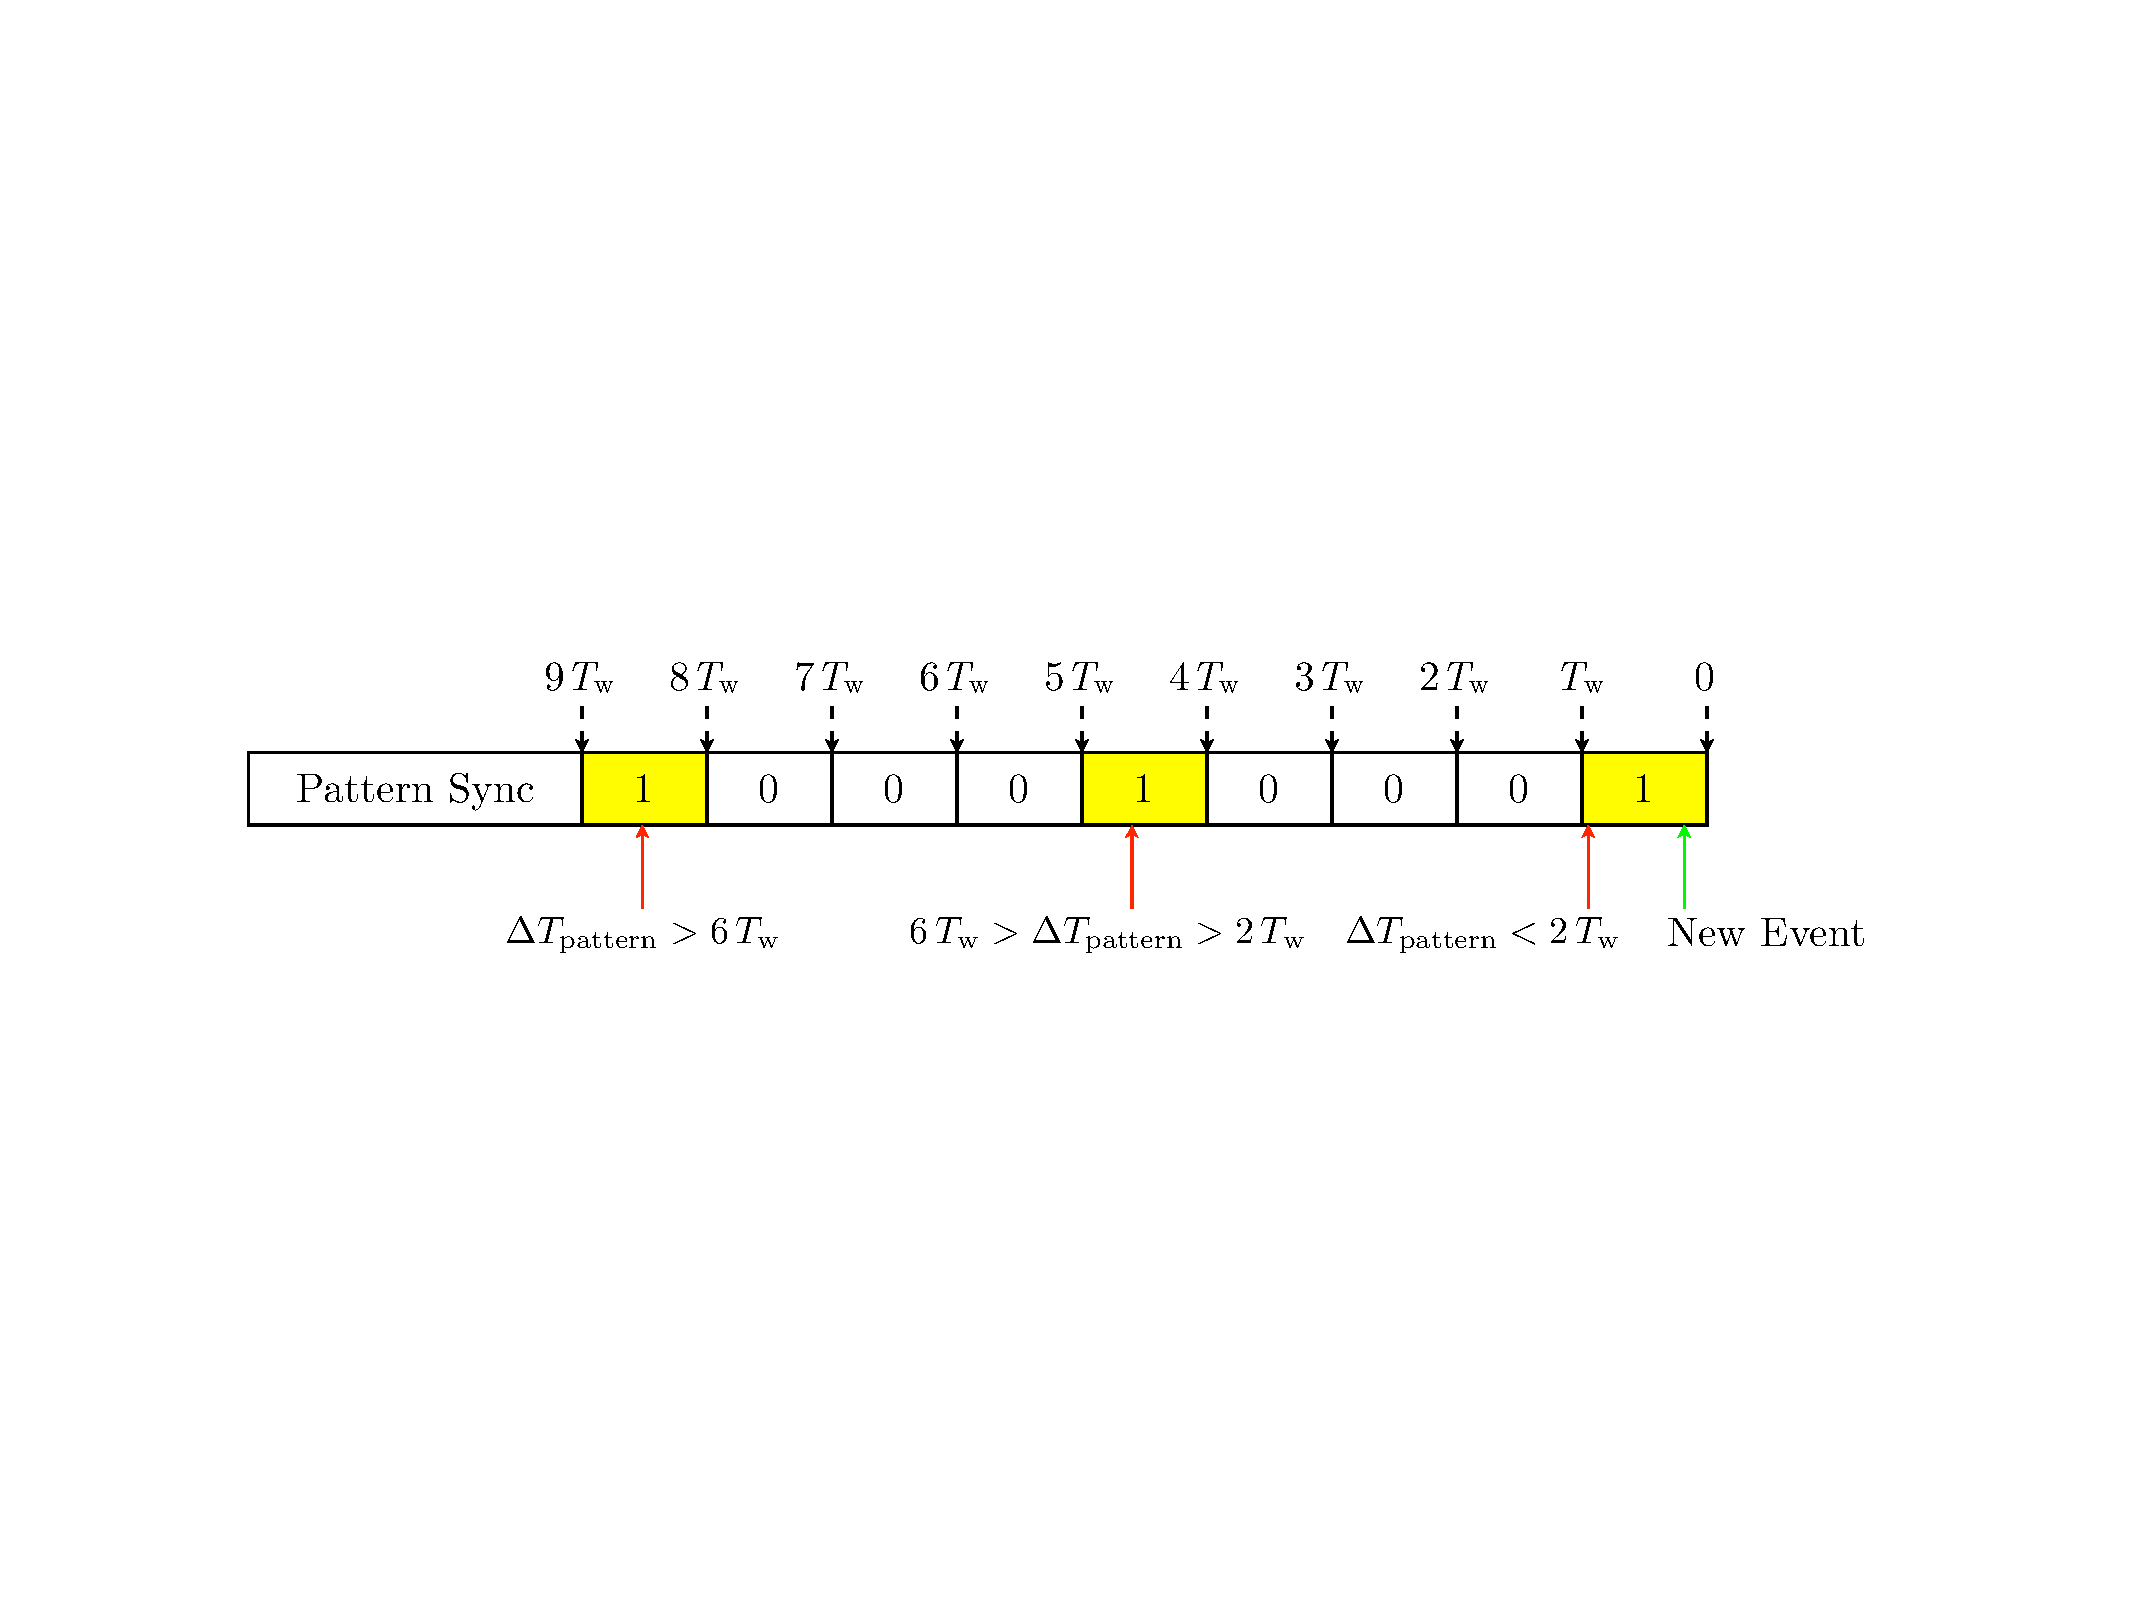
\includegraphics[width=0.85\textwidth]{figs/tir-helicity-seed.pdf}
  \caption[Determine the radom seed for TIR helicity.]{Thresholds on $\dtpat$ to determine whether a Pattern Sync window is missed or not if the new event is a Pattern Sync event. Here $\tw$ is the time length of a helicity window in unit of scaler counts. The red arrows are different possibilities of the previous event. Yellow backgrounds indicate the possible range of $\dtpat$, and the thresholds are set in between these ranges to avoid any possible error due to scaler fluctuation. \label{A1S2SS2F2}}
\end{figure}

Once the random seed is generated, the second step is to predict the reported and the actual helicity for each event with the seed. Since the random seed needs to be left-shifted by 1 bit whenever a helicity quartet is finished, it is critical to determine $n$, the number of missed Pattern Sync windows. Besides $\dtpat$, another time interval $\dt$ is used to determine $n$. Assuming the time-stamp of the previous event is $\tlast$, $\dt$ can be expressed as $\dt=T-\tlast$. The random seed must be left-shifted by $n$ bits before making the helicity prediction as described below. When shifting, the new bits are always calculated with the algorithm in \Cref{A1S2F1}. Due to the particularity of the Pattern Sync event, three different situations need to be considered separately:
\begin{enumerate}[parsep=0pt]
\item \label{A1S2SS2A3} Both the new event and its previous event are Pattern Sync events. In this case, the restrictions on $\dtpat$ shown in \Cref{A1S2SS2F2} still works. If $\dtpat<2\tw$, the new event is in the same window of the previous one. The same random seed is used to predict the actual helicity. If $(4\times n+2)\tw<\dtpat<(4\times n+6)\tw$, $n$ Pattern Sync windows are missed ($n$ can be 0). The random seed is left-shifted by $n$ bits, then the prediction for the new event is made. After the prediction, the seed is left-shifted by 1 bit to prepare for the next prediction.
\item \label{A1S2SS2A4} The new event is a Pattern Sync event but its previous event is not. In this case, the time interval $\dt$ is used to determine $n$, the number of missed Pattern Sync windows, as $n=\mathrm{int}[\dt/(4\tw)]$. The random seed is left-shifted by $n$ bits, then the prediction for the new event is made. After the prediction, the seed is left-shifted by 1 bit to prepare for the next prediction.

\begin{table}[b!]
  \centering
  \newcolumntype{C}[1]{>{\centering\arraybackslash}m{#1}}
  \begin{tabular}{|C{1.7cm}|C{1.4cm}|C{1cm}|C{1.5cm}|C{1.7cm}|C{1.4cm}|C{1cm}|C{1.5cm}|}
    \hline
    \multicolumn{4}{|c|}{Prediction of the First Window is $+$} & \multicolumn{4}{c|}{Prediction of the First Window is $-$} \\ \hline
    Reported Helicity & Pattern Sync & Pair Sync & Actual Helicity & Reported Helicity & Pattern Sync & Pair Sync & Actual Helicity \\ \hline
    1 & 1 & 1 & $+$ & 1 & 1 & 1 & $-$ \\ \hline
    0 & 0 & 0 & $-$ & 0 & 0 & 0 & $+$ \\ \hline
    0 & 0 & 1 & $-$ & 0 & 0 & 1 & $+$ \\ \hline
    1 & 0 & 0 & $+$ & 1 & 0 & 0 & $-$ \\ \hline
    0 & 1 & 1 & $+$ & 0 & 1 & 1 & $-$ \\ \hline
    1 & 0 & 0 & $-$ & 1 & 0 & 0 & $+$ \\ \hline
    1 & 0 & 1 & $-$ & 1 & 0 & 1 & $+$ \\ \hline
    0 & 0 & 0 & $+$ & 0 & 0 & 0 & $-$ \\ \hline
  \end{tabular}
  \caption[The corresponding actual helicity for a helicity pattern.]{Find the actual helicity of a event according to its reported helicity and Pair Sync value. \label{A1S2SS2T1}}
\end{table}

\item The new event is not a Pattern Sync event. In this case, the time interval $\dtpat$ is used to determine $n$ as $n=\mathrm{int}[\dtpat/(4\tw)]$. The random seed is left-shifted by $n$ bits, then the prediction for the new event is made. But in this case, the prediction only tells the actual helicity of the first window in the Quartet pattern to which the new event belongs to. The actual helicity of this particular event can be determined according to its Pattern Sync, Pair Sync and the reported helicity value, as shown in \Cref{A1S2SS2T1}. Unlike cases \ref{A1S2SS2A3} and \ref{A1S2SS2A4}, the seed does not need to be left-shifted after the prediction, but the $\tlastpat$ need to be increased by $n\times4\tw$ in case the next event is still not a Pattern Sync event.
\end{enumerate}

\Cref{A1S2SS2F3} illustrates the thresholds on $\dt$ and $\dtpat$ to determine $n$ for these 3 situations. The prediction of the reported helicity of each event is checked with the reported helicity written in the raw data file. If the prediction fails, all events in this quartet are marked as bad. The 30-bit random seed is reset and regenerated.

\begin{figure}[tb!]
  \centering
  \begin{subfigure}[t]{\textwidth}
    \centering
    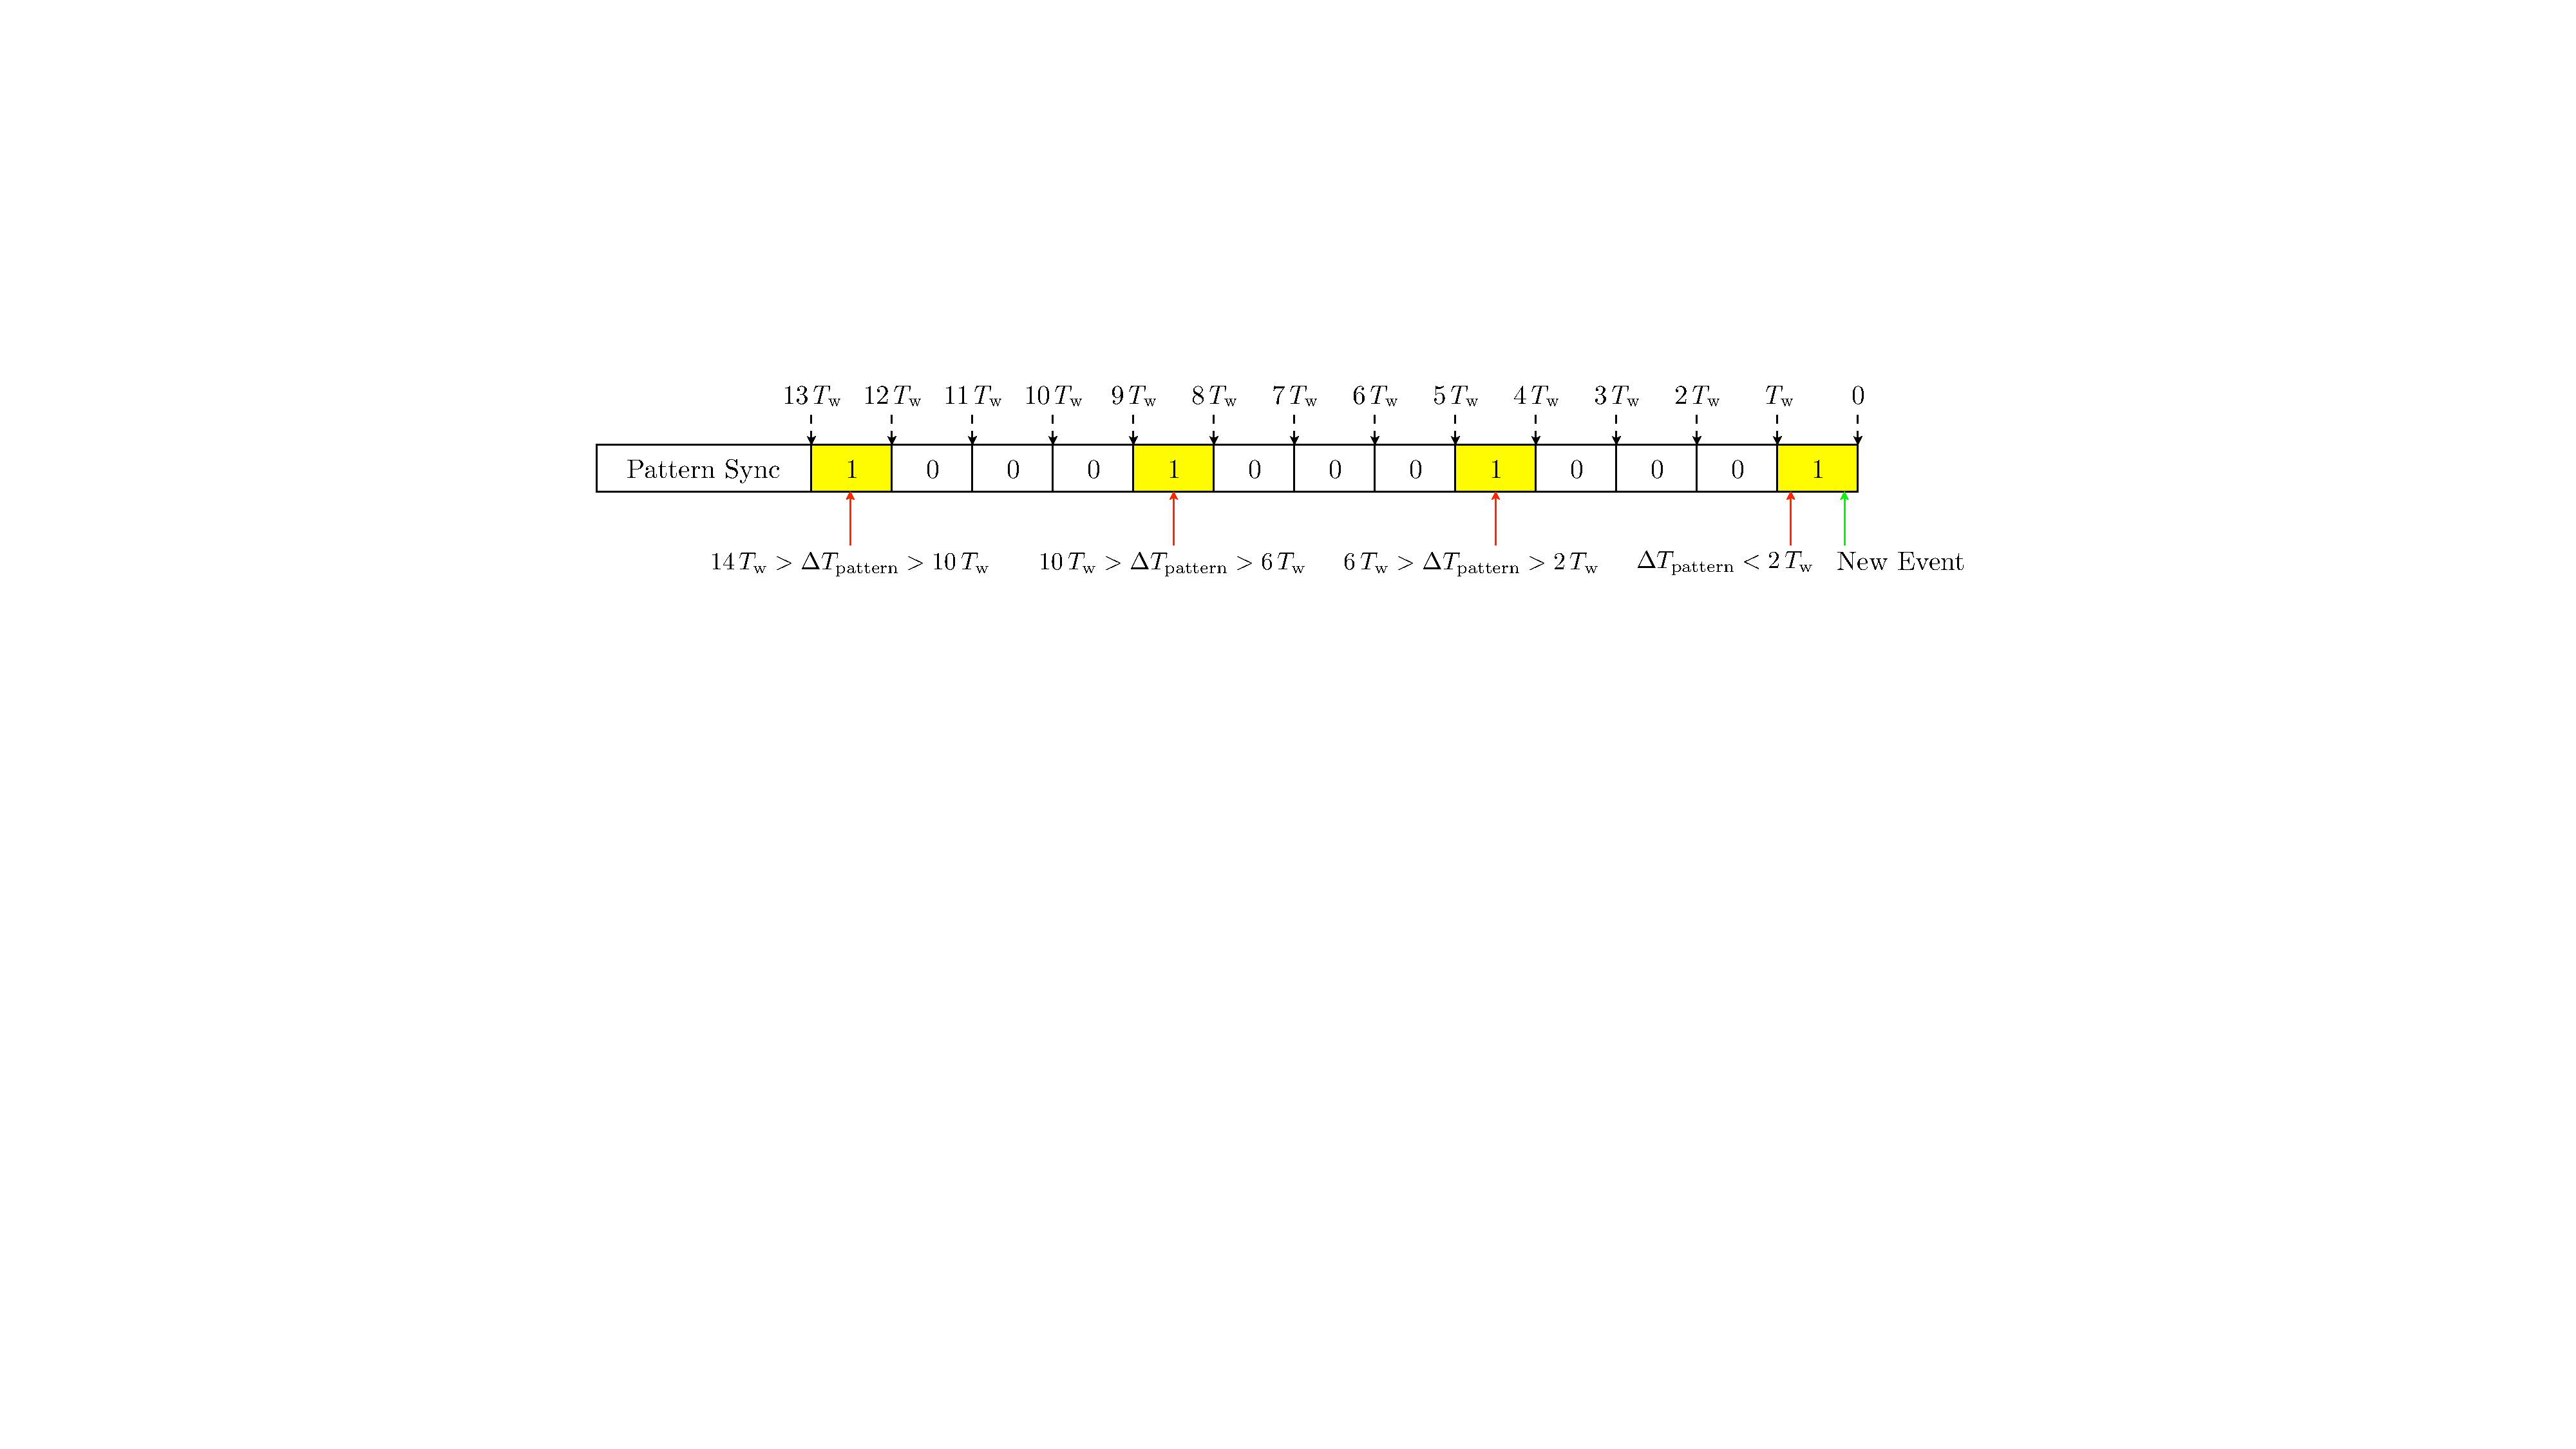
\includegraphics[width=\textwidth]{figs/tir-helicity-prediction-a.pdf}
    \caption{\label{A1S2SS2F3a}}
  \end{subfigure}
  \begin{subfigure}[t]{\textwidth}
    \centering
    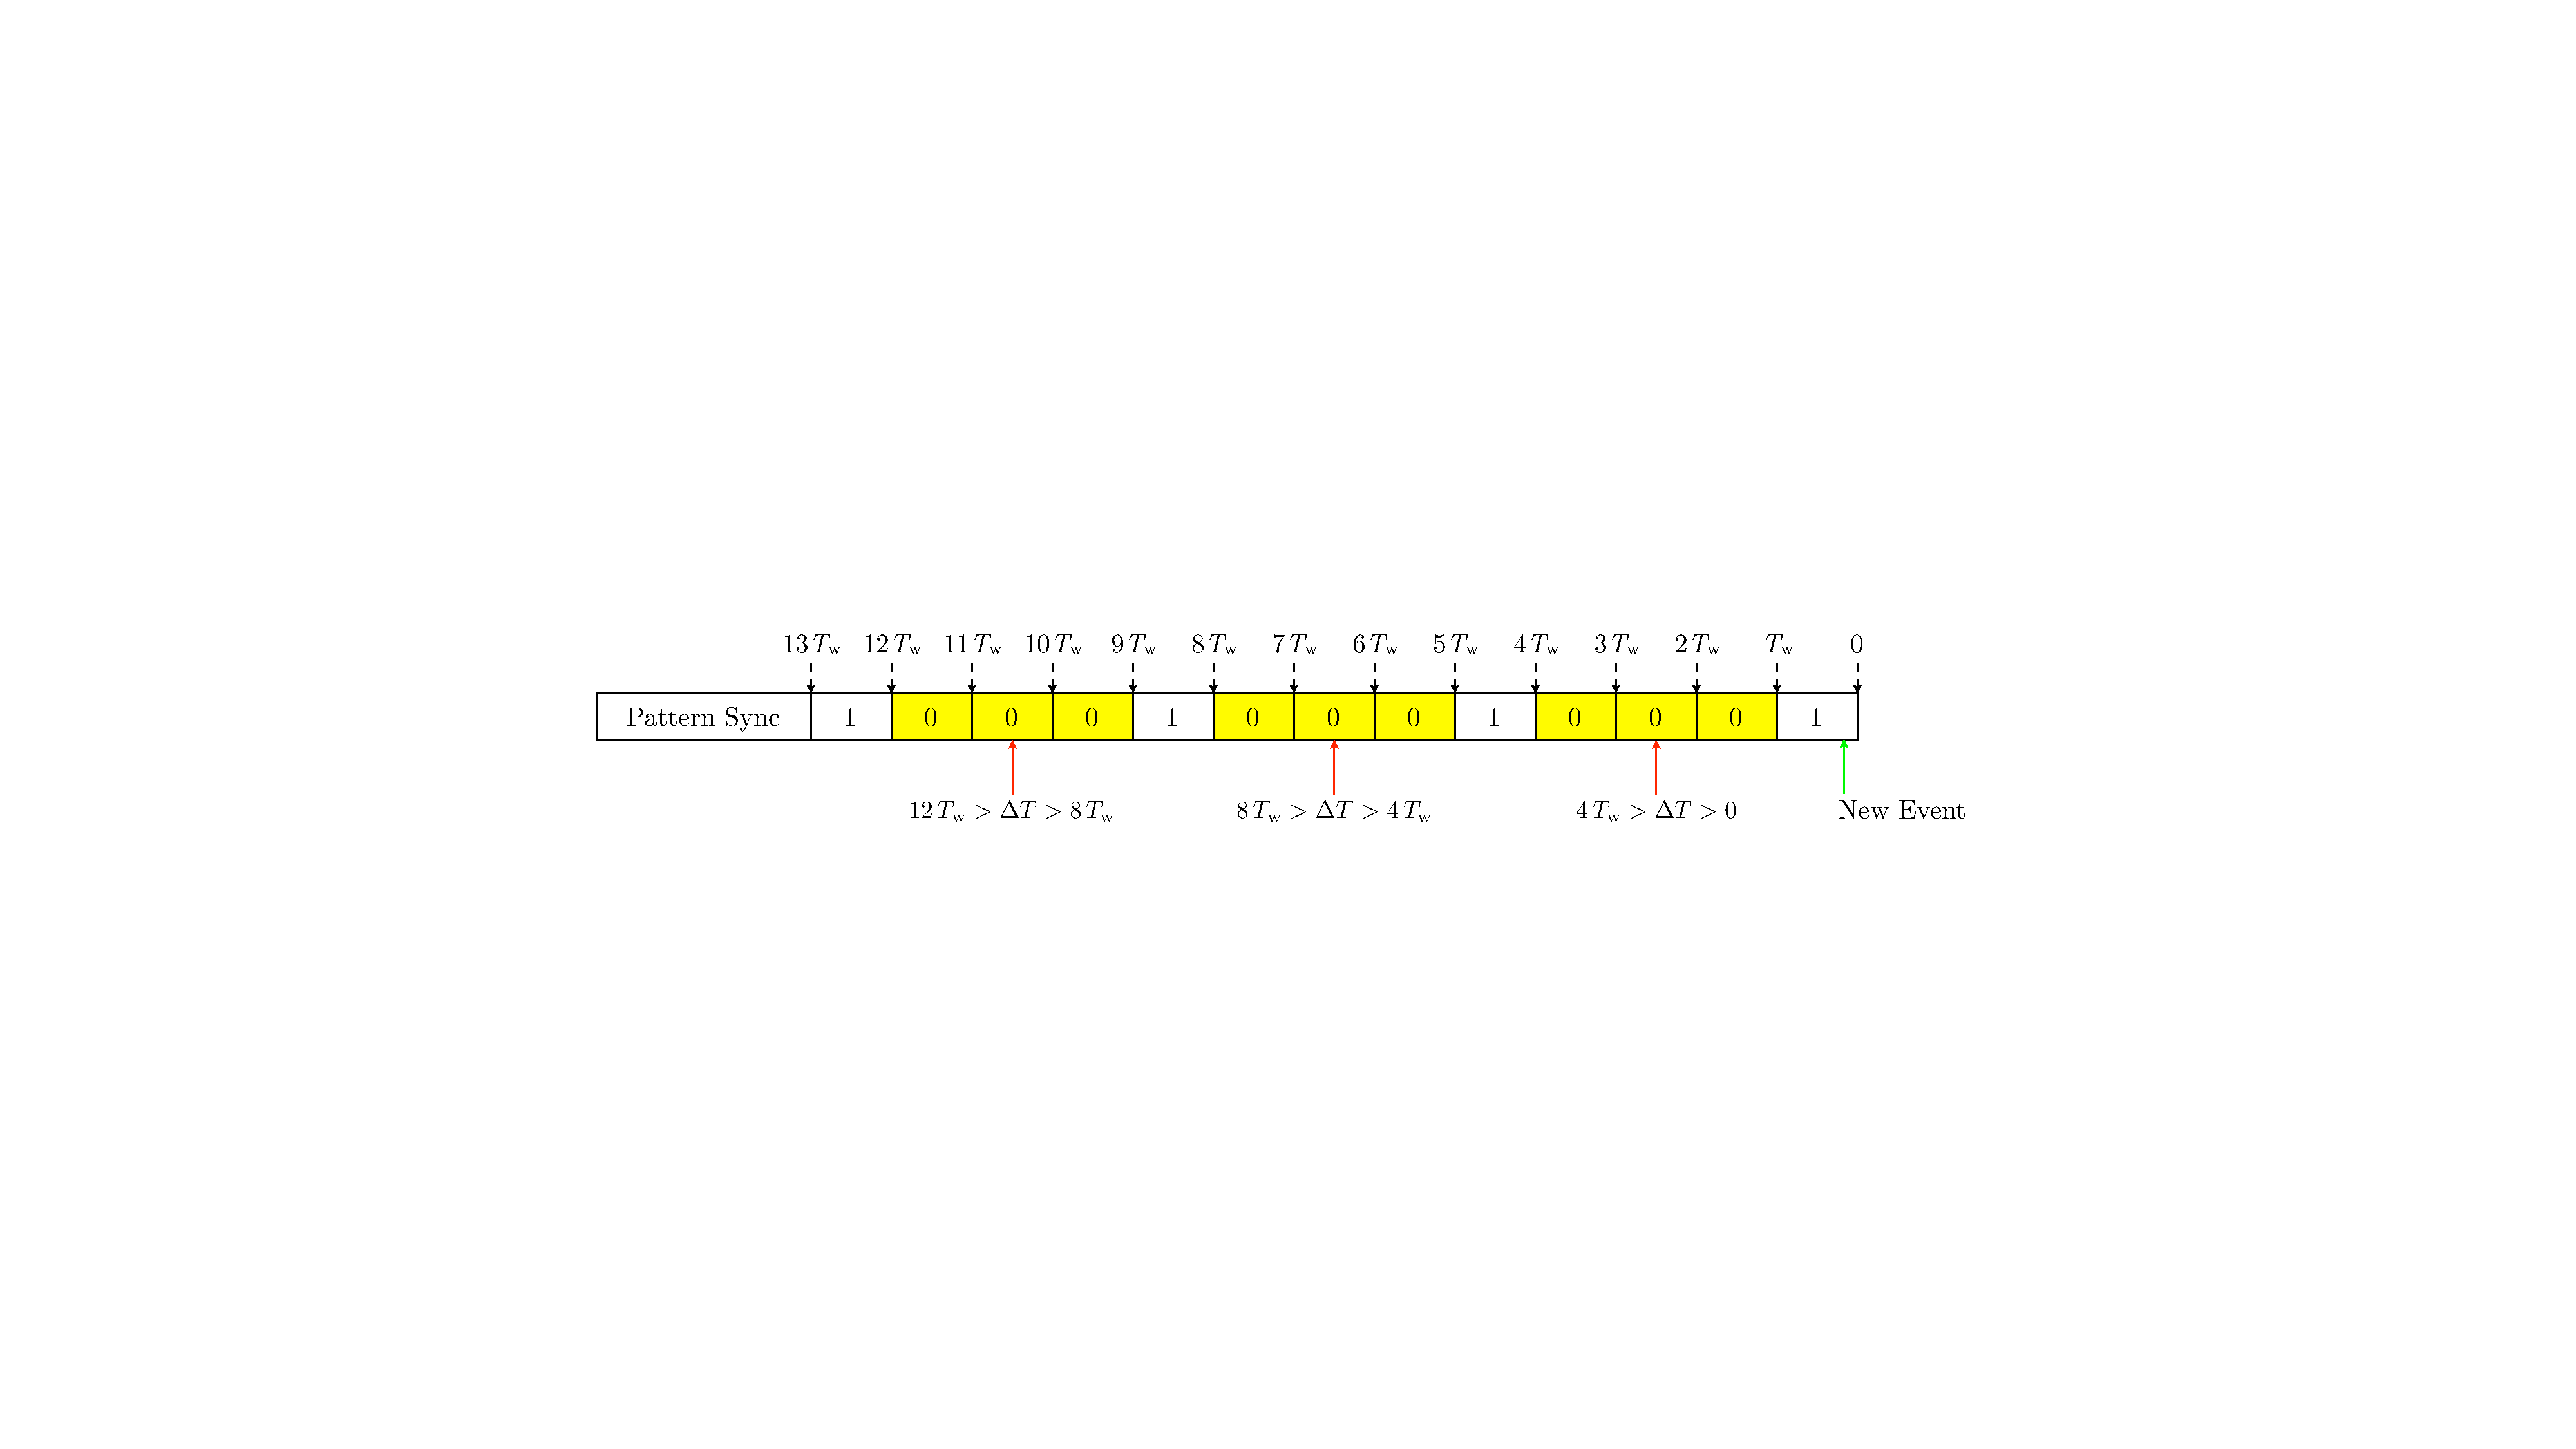
\includegraphics[width=\textwidth]{figs/tir-helicity-prediction-b.pdf}
    \caption{\label{A1S2SS2F3b}}
  \end{subfigure}
  \begin{subfigure}[t]{\textwidth}
    \centering
    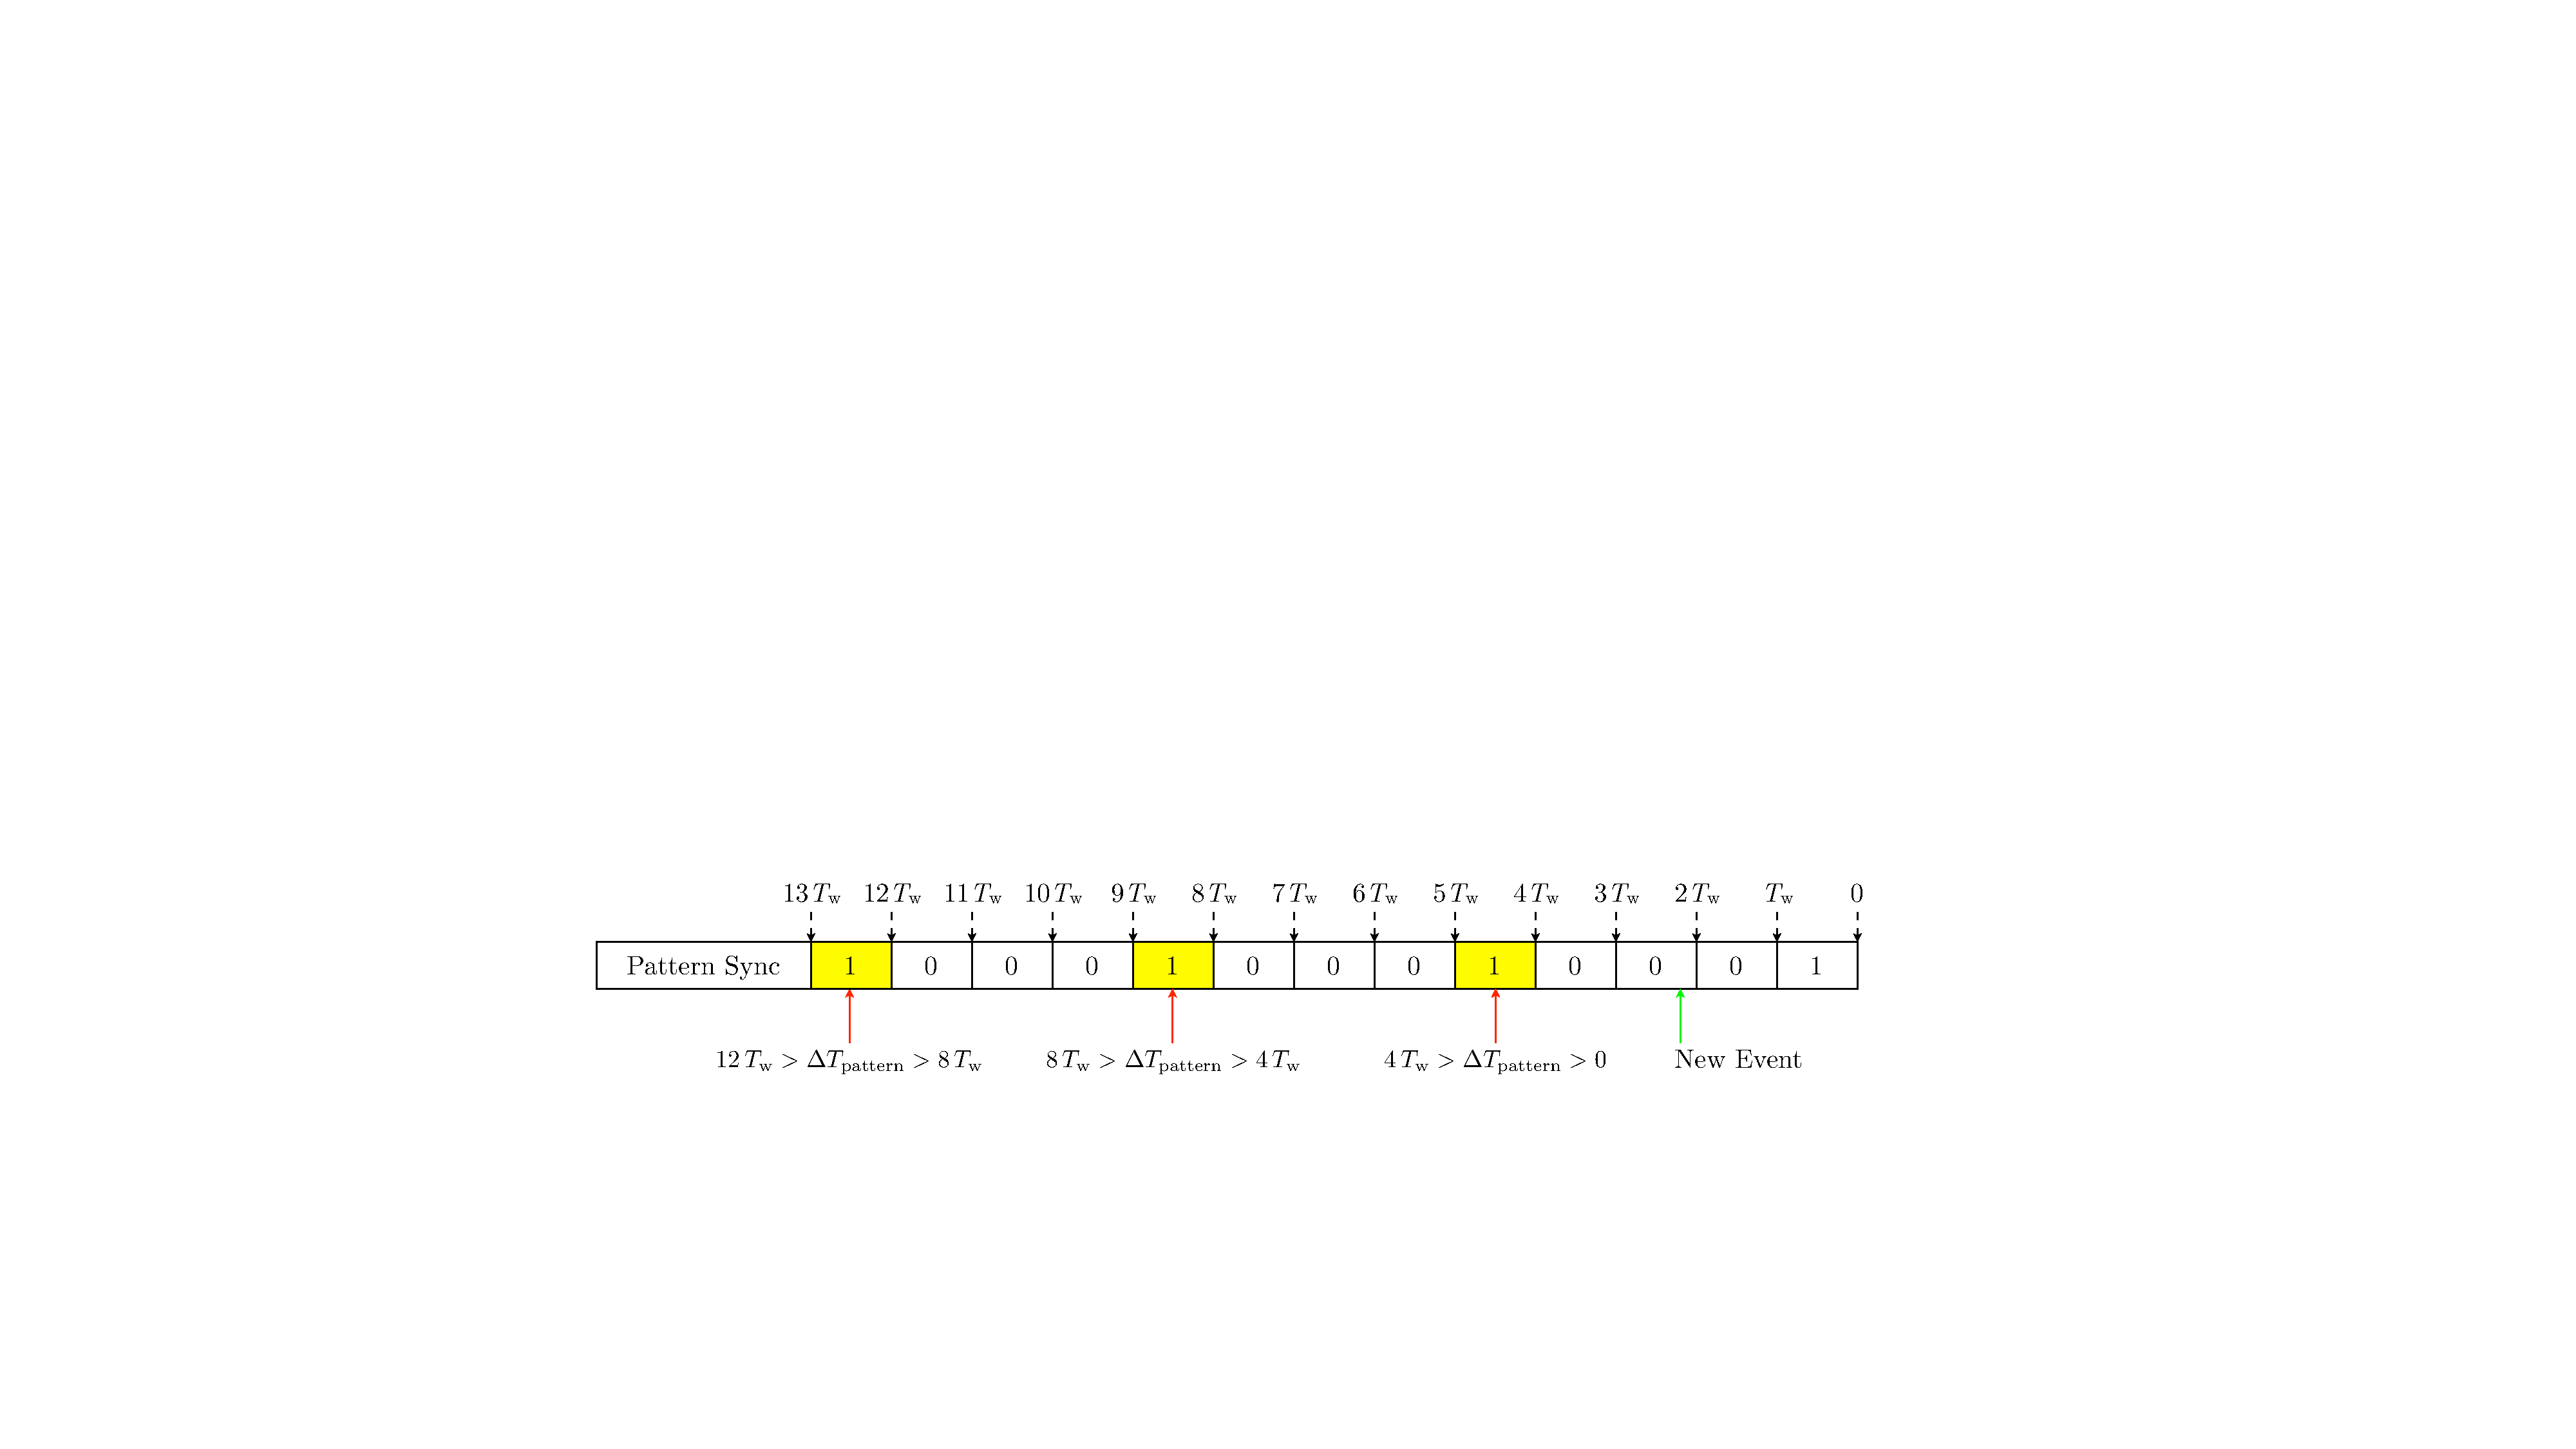
\includegraphics[width=\textwidth]{figs/tir-helicity-prediction-c.pdf}
    \caption{\label{A1S2SS2F3c}}
  \end{subfigure}
  %\captionsetup{skip=0ex}
  \caption[Predict actual TIR helicity.]{Thresholds to determine the number of missed Pattern Sync windows: (a) Both the new event and its previous event are Pattern Sync events; (b) The new event is a Pattern Sync event but its previous event is not one; (c) The new event is not a Pattern Sync event. Yellow backgrounds indicate all possible time ranges for the previous event. And the thresholds are chosen in between the possible ranges of $\dt$ and $\dtpat$. \label{A1S2SS2F3}}
\end{figure}

Due to the fluctuation of the scaler, the time interval $\dt$ and $\dtpat$ may not always satisfy the thresholds described and in \Cref{A1S2SS2F3}. The excluded $\tsettles$ events are used to calibrate $\tlast$ and $\tlastpat$ since the time length of helicity windows is fixed. As shown in \Cref{A1S2SS2F4}, a $\tsettles$ event which is right before a Pattern Sync window is selected for calibration. Assuming the time-stamp of this $\tsettles$ event is $T$, the $\tlast$ is set to $T-\tw$ and the $\tlastpat$ is set to $T-3\tw$. Once calibrated, $\tlast$ and $\tlastpat$ are not used to store the time stamp of previous events any more. The values of $\tlast$ and $\tlastpat$ are increased by $n\times4\tw$ if $n$ patterns are finished during the prediction. And any qualified $\tsettles$ events are used to recalibrate their values. The fluctuation of $\dt$ and $\dtpat$ is reduced by at least half if calculated with calibrated $\tlast$ and $\tlastpat$, the number of missed Pattern Sync windows can be determined more accurately, and the fail rate of the helicity prediction is reduced.

\begin{figure}[tb!]
  \centering
  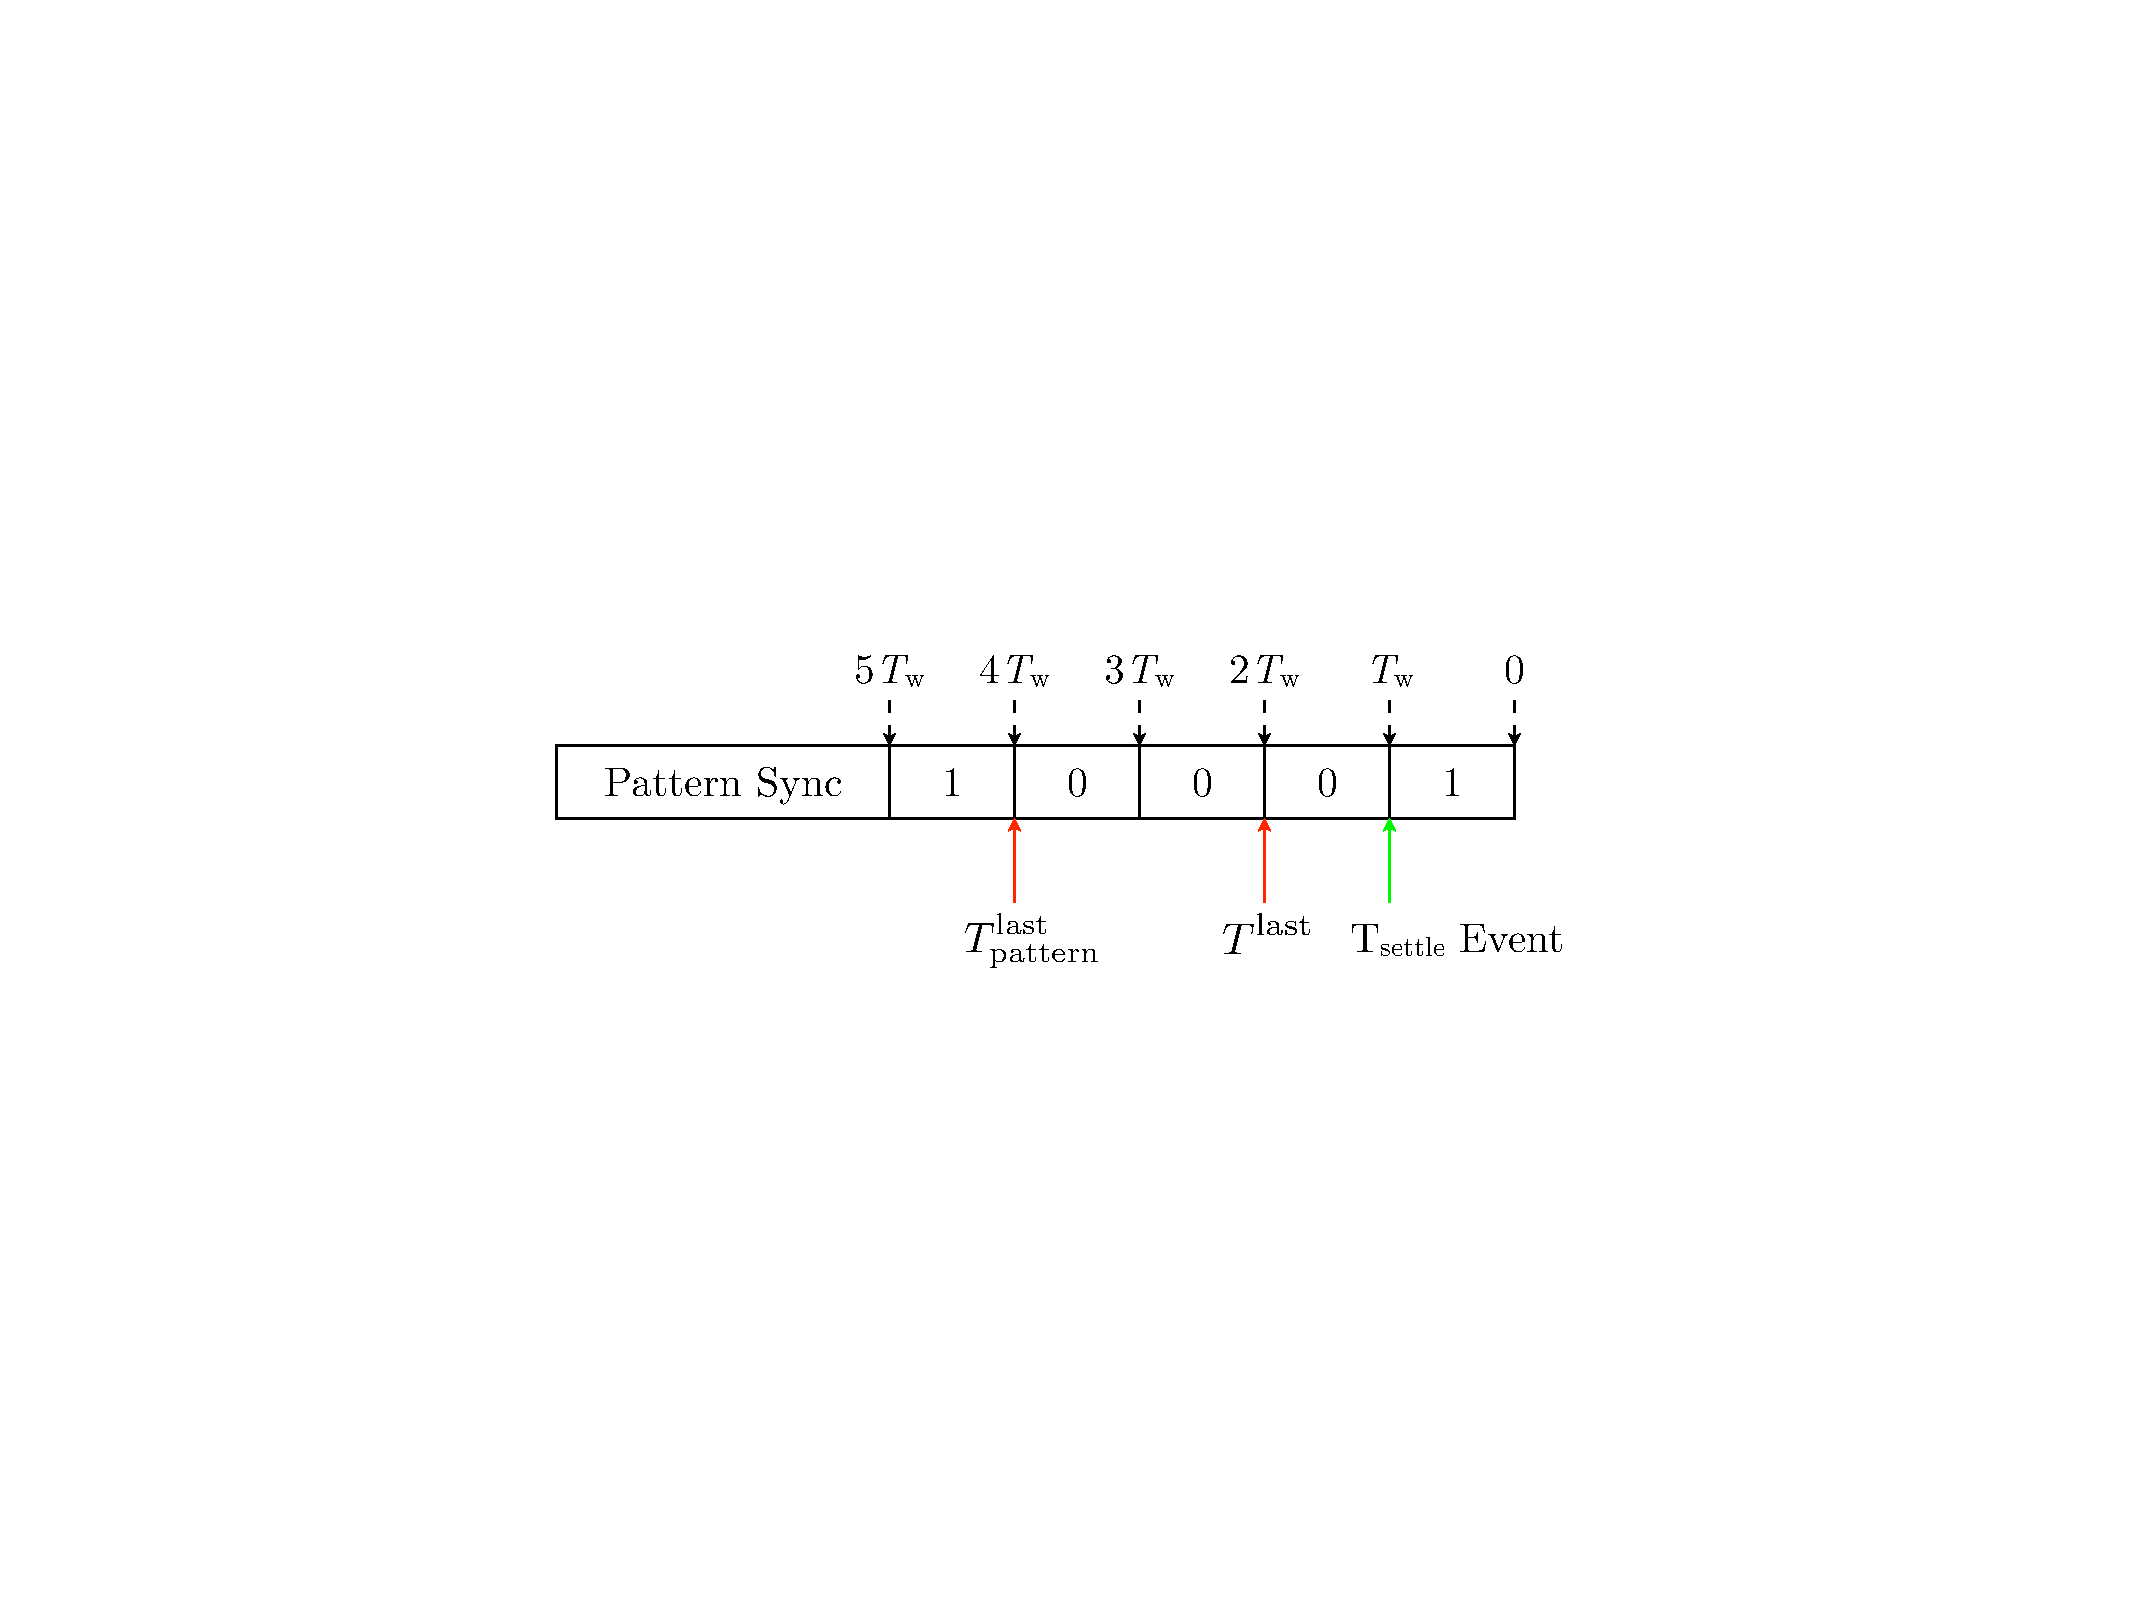
\includegraphics[width=0.5\textwidth]{figs/tir-helicity-tsettle-calibration.pdf}
  \caption{Calibrate $\tlast$ and $\tlastpat$ with $\tsettles$ events. \label{A1S2SS2F4}}
\end{figure}

\subsection{Align TIR Helicity with Ring Buffer Helicity}
\label{A1S2SS3}

The purpose to align TIR helicity with ring buffer helicity is to insert the helicity-gated informations into the physical data stream. As mentioned in \Cref{A1S2F1}, the helicity random seed repeats every $2^{30}$-1 bits, thus it never repeats repeats during one particular run, which is usually hour-long. Therefore the random seed can be used as the ``fingerprint'' to do this alignment.

Before alignment, the quality of the prediction result is checked to avoid false asymmetry. If the actual helicity of a event is not predictable due to some error, events in the same helicity quartet are also marked as bad during the checking. For the ring buffer helicity, the BCM information is used to determine beam trips. The data taken during the beam trip and within 30 helicity quartets before and after the beam trip is excluded from the data analysis to prevent any systematic error.

\begin{figure}[tb!]
  \centering
  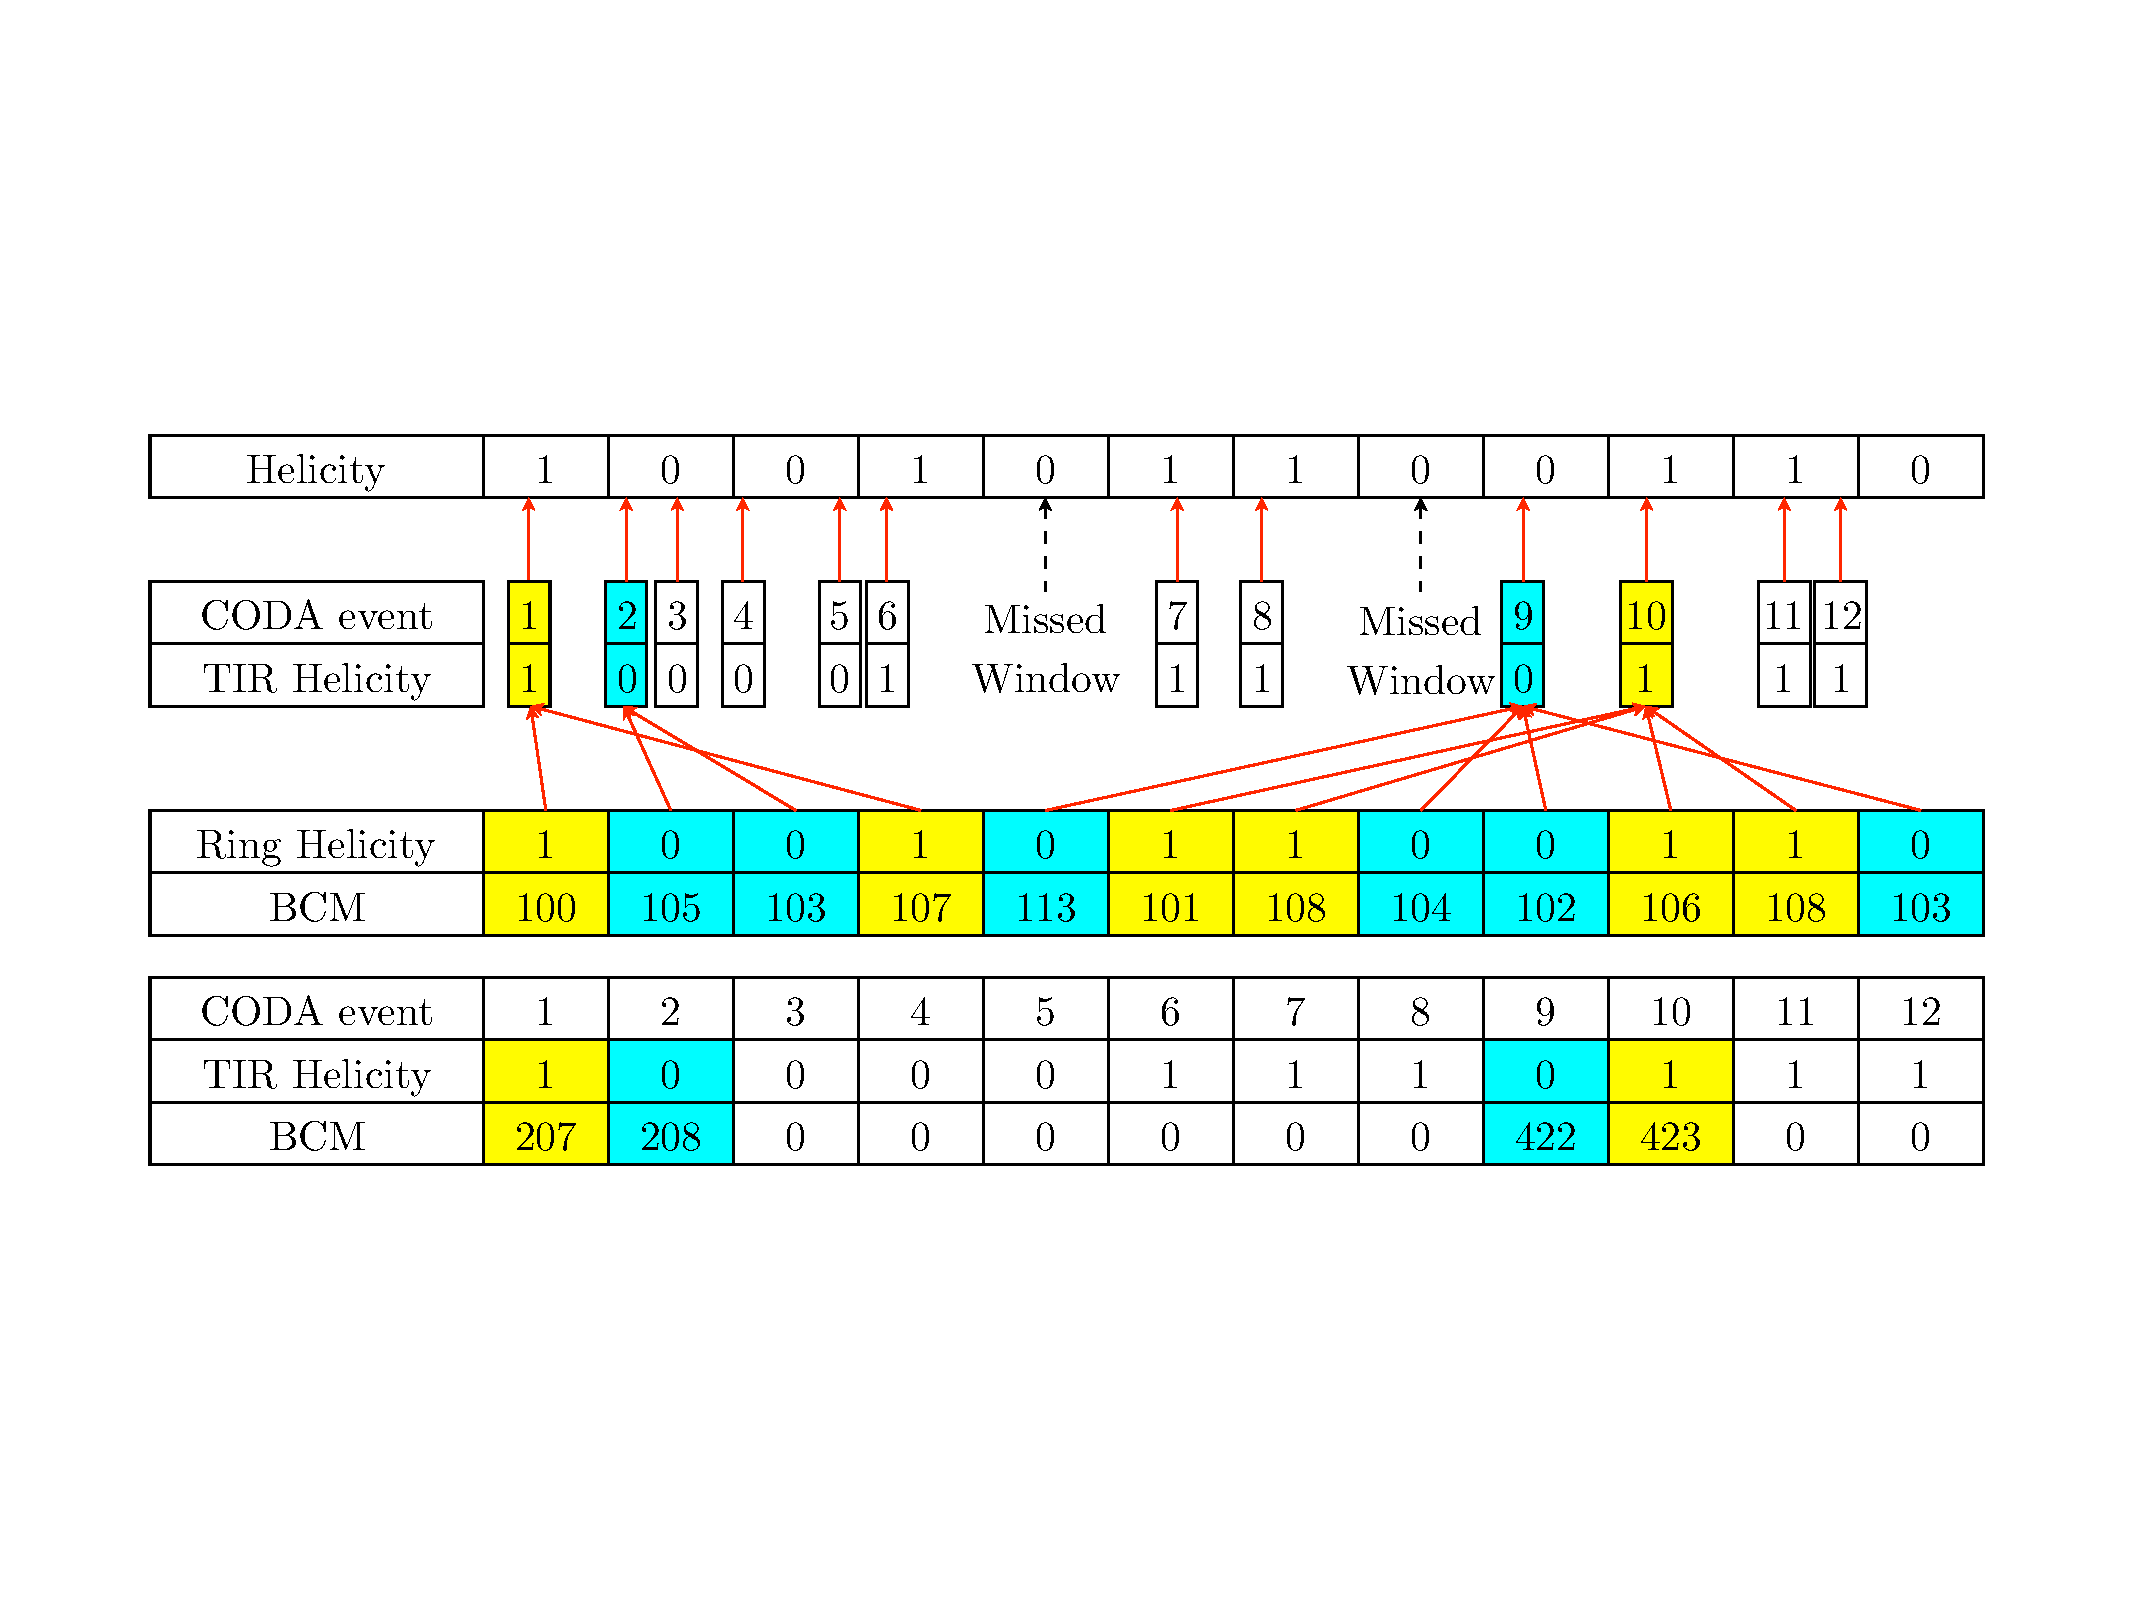
\includegraphics[width=\textwidth]{figs/helicity-align.pdf}
  \caption[Align TIR helicity with ring buffer helicity.]{Align TIR helicity with ring buffer helicity. Take BCM as an example of the helicity-gated data. The second quartet in the helicity sequence missed two 0 helicity windows, so the BCM values of this pattern is added to the values of the next quartet to be saved in the physical event stream. \label{A1S2SS3F1} }
\end{figure}

\Cref{A1S2SS3F1} shows an example of the alignment. Here BCM is selected as an example of the helicity-gated data. For each helicity quartet in the ring buffer helicity, two BCM values $C_{+}$ and $C_{-}$ are calculated for $+$ and $-$ helicity. The random seed saved for this pattern is compared with all the random seeds saved in the TIR helicity. If a matching pattern is found and the pattern contains at least one event with $+$ helicity and one event with $-$ helicity, $C_{+}$ is saved to the first event with $+$ helicity and $C_{-}$ is saved to the first event with $-$ helicity. If no pattern matches, $C_{+}$ and $C_{-}$ is added to the BCM values of the next helicity quartet in the ring buffer helicity. This method preserves the most helicity-gated data in the physical event stream so they can be used in helicity-related calculation.

\section{Test with Charge Asymmetry}
\label{A1S3}

The helicity decoder is tested with beam charge asymmetry during the experiment. The beam charge asymmetry $A_{Q}$ can be expressed as:
\begin{equation} \label{A1S3E1}
A_{Q}=\frac{Q_{+}-Q_{-}}{Q_{+}+Q_{-}}.
\end{equation}
Here $Q_{\pm}$ are the beam charge with helicity $\pm 1$. The beam charge asymmetry can be adjusted in the injector. For the test, beam with large charge asymmetry is required from the injector and is measured with HRS DAQ (SIS3801 scaler), Hall A M{\o}ller DAQ and Hall C DAQ simultaneously. The M{\o}ller DAQ and Hall C DAQ are used as reference of this test. The results of the test are listed in \Cref{A1S3T1}. The calculation result of the new helicity decoder agrees well with the M{\o}ller DAQ and Hall C DAQ, indicating our new decoder can be used for the analysis.

\begin{table}[h!]
  \centering
  \begin{tabular}{|*{7}{c|}}
    \hline
    ID & Left HRS & Right HRS & Moller & Hall C \\ \hline
    1 & -0.91\% & -0.91\% & -0.92\% & -0.91\% \\ \hline
    2 & -0.56\% & -0.56\% & -0.56\% & -0.56\% \\ \hline
    3 & -0.092\% & -0.095\% & -0.090\% & -0.094\% \\ \hline
  \end{tabular}
  \caption{Beam charge asymmetry test with different DAQs. \label{A1S3T1}}
\end{table}

\clearpage
\newpage

%%%%%%%%%%%%%%%%%%%%%%%%%%%%%%%%%%%%%%%%%%%%%%%%%%%%%%%%%%%%%%%%%%%%%%
% -*-latex-*-
